\documentclass[a4paper,11pt]{ltjsreport}
\usepackage{luatexja}
\usepackage[no-math,deluxe,expert]{luatexja-preset}
\usepackage[top=1.47cm, bottom=1.7cm, left=1.6cm, right=1.6cm]{geometry}
\usepackage{authblk}
\usepackage[
  luatex,
  pdfencoding=auto,
  psdextra,
  pdfversion=1.7,
  hidelinks,
  pdfa,
  unicode=true
]{hyperref}
\usepackage{hyperxmp}
\usepackage[luatex]{graphicx}
\usepackage[table]{xcolor}
\usepackage{epstopdf}
\usepackage{colortbl}
\usepackage{svg}
\usepackage{subcaption}
\usepackage{dirtree}
\usepackage{listings}
\usepackage{siunitx}
\usepackage{float}
\usepackage{ascmac}
\usepackage{minted}
\usepackage{amsmath}
\usepackage{mathtools}
\usepackage[warnings-off={mathtools-colon,mathtools-overbracket}]{unicode-math}
\usepackage{csvsimple}

\title{フィッシングメール観察中の視線位置}
\author{青木汰一, 阿部真咲, 田村昂瑛, 三浦孝一郎, 渡邊湊至}
\hypersetup{
  pdftitle={フィッシングメール観察中の視線位置},
  pdfsubject={生体情報処理の体験,時系列データ処理演習.},
  pdfkeywords={情報処理実習, J23, 眼球運動, アイトラッキング, フィッシングメール},
  pdfauthor={青木汰一, 阿部真咲, 田村昂瑛, 三浦孝一郎, 渡邊湊至},
  pdfcopyright={The Wayama Lab 2023.},
  pdfcontactcity={Ichinoseki},
  pdfcontactregion={Iwate},
  pdfcontactpostcode={021-8511},
  pdfcontactcountry={Japan},
  pdflang={ja-JP},
  pdfmetalang={ja-JP},
  pdfcaptionwriter={Koyo Tamura},
  pdfcreationdate={2023-12-4},
  pdfmetadate={2023-12-4},
  pdfmoddate={2023-12-11},
  pdfdisplaydoctitle=true,
  draft=false,
  pdfapart=3,
  pdfaconformance=u,
  keeppdfinfo,
}

\newenvironment{code}{\captionsetup{type=listing}}{}
\captionsetup[listing]{name=ソースコード}
% Default fixed font does not support bold face
\DeclareFixedFont{\ttb}{T1}{txtt}{bx}{n}{12} % for bold
\DeclareFixedFont{\ttm}{T1}{txtt}{m}{n}{12}  % for normal
% Custom colors
\definecolor{deepblue}{rgb}{0,0,0.5}
\definecolor{deepred}{rgb}{0.6,0,0}
\definecolor{deepgreen}{rgb}{0,0.5,0}
\epstopdfsetup{suffix=.eps,}

\immediate\pdfobj stream attr{/N 3} file{sRGB.icc}
\pdfextension catalog{
  /OutputIntents [
    <<
      /Type /OutputIntent
      /S /GTS_PDFA1
      /DestOutputProfile \the\pdflastobj\space 0 R
      /OutputConditionIdentifier (sRGB)
      /Info (sRGB)
    >>
  ]
}

\pdfvariable omitcidset=1
\begin{document}
\begin{titlepage}
	\begin{center}
		{\Large 【情報処理実習II[J23]】}
		\vspace{5truept}

		{\LARGE レポート課題}
		\vspace*{70truept}

		{\Huge フィッシングメール観察中の視線位置}
		\vspace{10truept}

		{\LARGE Gaze position while observing phishing e-mails}
		\vspace{40truept}

		{\large 指導教員}
		\vspace{5truept}

		{\Large 宇梶 郁}
		\vspace{120truept}

		\begin{table}[H]
			\centering
			\Large
			\begin{tabular}{rcll}
				1  & f20001 & 青木 汰一  & Taichi Aoki    \\
				4  & f20007 & 阿部 真咲  & Masaki Abe     \\
				36 & f20113 & 田村 昂瑛  & Koyo Tamura    \\
				45 & f20145 & 三浦 孝一郎 & Koichiro Miura \\
				49 & f20159 & 渡邊 湊至  & Soji Watanabe
			\end{tabular}
		\end{table}
		\vspace{50truept}

		{\Large 一関工業高等専門学校}

		{\Large 未来創造工学科 情報・ソフトウェア系 和山研究室}
		\vspace{10truept}

		{\large The Wayama Lab, Division of Computer Engineering and Informatics,

			National Institute of Technology Ichinoseki College}
		\vspace{40truept}

		%{\Large 4年36番 f20113}
		%\vspace{60truept}

		{\Large 2023/12/11}
	\end{center}
\end{titlepage}

\tableofcontents
\clearpage

\chapter{概要}
\section{アイトラッキング}
\subsection{アイトラッキングとは?}
アイトラッキング(Eye Tracking)は,人間の視線の動きを追跡・計測する技術や方法を指す.これは,目の動きを分析して,人がどの部分に視線を向けているかを理解するための手法である.アイトラッキングは,心理学,医学,広告,人間コンピュータインタラクション(HCI),マーケティング,デザインなどの様々な分野で利用されている.

\subsection{アイトラッキングの手法}
アイトラッキングは,様々なセンサーやカメラを使用して視線の動きを追跡する.一般的な手法には,赤外線を使用した眼球の反射を検出する方法や,特殊なメガネに取り付けられたカメラで瞳孔や視点を追跡する方法などがある.

\section{フィッシングメール}
この実習ではとくにフィッシングメール(標的型攻撃メール)を題材とする.近年,Webページを用いた通信販売やテレワークの増加に伴い,電子メールによるセキュリティインシデントが問題となっている.今回の実習ではフィッシングメール観察中の視線位置を解析することで下記の項目を検討する.\cite{jikkensho}

\begin{itemize}
	\item フィッシングメールを観察中に電子メールのどこを観察しているのか?
	\item フィッシングメールを見分けることができる人はどこを観察しているのか?
	\item フィッシングメールを見分けることができる人,できない人で視線位置に差があるのか?
\end{itemize}


\chapter{実験と仮説}
\section{目的}
本実験は,生体情報処理の体験,時系列データ処理演習および人間の行動と外界刺激の関係を考察するために行う.\cite{ukaji}

\section{実験内容}
以下,本実験書\cite{jikkensho}を引用したものである.

\subsection{実験設定}
眼球運動計測装置として「Tobii Pro スペクトラム」を使用.眼球運動計測装置の視線位置計測リフレッシュレートは120\si{\hertz}に設定した.また,実験プログラムは「Tobii Pro Lab」によって作成した.

呈示刺激として,Gmailの迷惑メールフィルタで迷惑メールと判定されたメールを使用した.メールファイルはメーラー(Thunderbird)で開き,そのスクリーンショットが刺激として呈示された.メール内のリンクは,そのURLをテキストボックスで明記した.

電子メールは15通呈示され,そのうち10通はフィッシングメールであり,5通は通常のメールである.

被験者は一関高専4J,5Sの学生だった.被験者は事前に実験についてインフォームドコンセントを受け,実験目的や実験の危険性について説明を受けた.実験に参加した被験者のうち1名(ID000)は実験者であり,今回の実験プログラムを作成した.

\subsection{手順}
\begin{enumerate}
	\item 被験者はディスプレイの前に座り,頭部をアゴ台に載せて固定.
	\item 電子メールの画像が呈示され,そのメールが怪しいメールかどうか判断し,カーソルキーで応答.
	\item 電子メールの画像を判断している最中の視線位置を眼球運動計測装置で計測.
	\item 実験開始時に眼球運動計測装置のキャリブレーションを実行.
	\item 眼球運動計測装置の計測データをtsvファイルにエクスポート.
\end{enumerate}
\clearpage
\section{計測データのまとめ}
Moodleより図\ref{fig:dirtree}のClass\_EyeTrackingフォルダをダウンロードする.

\begin{figure}[H]
	\begin{minipage}{0.3\linewidth}
		\hspace{1em}
	\end{minipage}
	\begin{minipage}{0.6\linewidth}
		\dirtree{%
			.1 \makebox[1.5ex][r]{\includesvg[width=0.25cm]{icons/folder.svg} Class\_EyeTracking}.
			.2 \includesvg[width=0.25cm]{icons/folder.svg} data.
			.3 \includesvg[width=0.25cm]{icons/file.svg} ID000\_DataExport.csv.
			.3 \includesvg[width=0.25cm]{icons/file.svg} ID---\_DataExport.csv.
			.3 \includesvg[width=0.25cm]{icons/file.svg} ID105\_DataExport.csv.
			.2 \includesvg[width=0.25cm]{icons/folder.svg} Metrics.
			.3 \includesvg[width=0.25cm]{icons/file.svg} ID000\_Metrics.tsv.
			.3 \includesvg[width=0.25cm]{icons/file.svg} ID---\_Metrics.tsv.
			.3 \includesvg[width=0.25cm]{icons/file.svg} ID105\_Metrics.tsv.
			.2 \includesvg[width=0.25cm]{icons/folder.svg} stimul.
			.3 \includesvg[width=0.25cm]{icons/photo.svg} 01\_Kyoumu\_T\_Stim.png.
			.3 \includesvg[width=0.25cm]{icons/photo.svg} --\_-----\_-\_Stim.png.
			.3 \includesvg[width=0.25cm]{icons/photo.svg} 15\_SMBC\_F\_Stim.png.
			.2 \includesvg[width=0.25cm]{icons/file.svg} CorrectAnswer.csv.
			.2 \includesvg[width=0.25cm]{icons/note.svg} Demo\_analysis.ipynb.
			.2 \includesvg[width=0.25cm]{icons/file.svg} results\_example.csv.
		}
	\end{minipage}
	\caption{データ構成\label{fig:dirtree}}
\end{figure}
dataフォルダには,各IDごとの計測データがある.行方向に計測時間(タイムスタンプ),列方向に視線位置や,キーボード入力などの各種情報(データラベル)が記録されている.以下に詳細を示す.
\begin{itembox}[l]{csv構成}
	\begin{small}
		\begin{itemize}
			\item Recording timestamp:  レコード中のタイムスタンプ [\si{\micro \second}]
			\item Recording date:       レコード月日
			\item Participant name:     被験者名
			\item Recording duration:   総レコード時間 [\si{\milli \second}]
			\item Recording resolution height:  データ分解能(高さ)[pix]
			\item Recording resolution width:   データ分解能(幅)[pix]
			\item Average calibration accuracy (pixels): キャリブレーション正確度 [pix]
			\item Average calibration precision SD (pixels): キャリブレーション精度 [pix]
			\item Event:                イベント(キーボード押し,刺激呈示など)
			\item Event value:          イベント詳細(どのキーボード入力か? どの刺激呈示か?など)
			\item Gaze point X:         視線位置(X方向)左上が [0, 0]
			\item Gaze point Y:         視線位置(Y方向)
			\item Presented Media name: 提示されていたメディア名(画像ファイル名など)
			\item Eye movement type:    眼球運動の分類
			      \begin{itemize}
				      \item Fixation:     固視
				      \item Saccade:      サッケード(見たい物を網膜中心で捉えるための急速眼球運動)
				      \item EyesNotFound: 眼球が観測てきていない(瞬きやキャリブレーション精度が悪いために生じる)
			      \end{itemize}
		\end{itemize}
	\end{small}
\end{itembox}

stimuliフォルダには,今回実験で用いた15枚のpng形式の画像データが格納されている.(図\ref{fig:a1}〜\ref{fig:a15})

\section{仮説}
\subsection{視線追跡の特徴}
フィッシングメールと通常のメールを区別する際,被験者の視線は特定のキーワードやリンクに集中すると予想される.Durationが大きい人ほどその傾向が強いのではないだろうか.また,メールのヘッダーを見る人,ハイパーリンクのリンク先を見る人はそうでない人に比べ正答率が高くなっているのではないか.

\subsection{Durationの違い}
フィッシングメールは疑わしい要素を含むため,被験者がこれらのメールを読むのには,通常のメールに比べDurationが大きくなっていると予測される.

\section{検証に用いる分析データ}
今回前項で立てた仮説を検証するために提供データを分析し,以下のものを用意する.
\begin{itemize}
	\item $TP, FP, FN, TP$それぞれを記録したデータと,それを用いて計算した各指標\footnote{$Accuracy, Precision, Recall, F\textrm{-}measure$}.
	\item 実験中に呈示画像に興味がある時間帯「Time of Interest (ToI)」.
	\item 視線位置をプロットし,ヒートマップとして合成した画像.
	\item 視線が呈示刺激のどこにいたのかを示す「Area of Interest (AoI)」.
	\item 各値,指標のそれぞれの相関を示す係数.
\end{itemize}

\chapter{検証結果と考察}
\section{出力データと画像}
\subsection{各指標}
各IDに対する正答率や指標を表\ref{confusion}に示す.
\begin{table}[H]
	\centering
	\rowcolors{2}{gray!15}{white}
	\resizebox{\textwidth}{!}{%
		\csvautotabular{results_example.csv}
	}
	\caption{各指標\label{confusion}}
\end{table}

\subsection{画像に対する正答率}
各画像に対する正答率を表\ref{imgacc}に示す.
\begin{table}[H]
	\centering
	\rowcolors{2}{gray!15}{white}
	\csvautotabular{imgacc.csv}
	\caption{画像ごとの正答率\label{imgacc}}
\end{table}

\subsection{ToI}
各IDのToIを表\ref{tabletoi}に示す.
\begin{table}[H]
	\centering
	\resizebox{\textwidth}{!}{%
		\begin{tabular}{|l|*{15}{r|}>{\columncolor{gray!15}}l|}
			\hline
			\rowcolor{gray!15}
			ID       & 01T       & 02F        & 03F       & 04F      & 05T       & 06F        & 07T         & 08F       & 09F      & 10T       & 11F        & 12F         & 13T        & 14F       & 15F        & Avg.        \\
			\hline
			\csvreader[
				head to column names,
			late after line=                                                                                                                                                                                                  \\\hline
			]{toi.csv}{}
			{%
			\csvcoli & \csvcolii & \csvcoliii & \csvcoliv & \csvcolv & \csvcolvi & \csvcolvii & \csvcolviii & \csvcolix & \csvcolx & \csvcolxi & \csvcolxii & \csvcolxiii & \csvcolxiv & \csvcolxv & \csvcolxvi & \csvcolxvii
			}
			\hline
		\end{tabular}
	}
	\caption{Time of Interest\label{tabletoi}}
\end{table}

\subsection{画像の正答率による比較}
\label{sec:imgacccompare}
表\ref{imgacc}より,正答率が最高の画像11\_LINE\_Fと最低の12\_Kyufu2\_F,15\_SMBC\_Fの3枚を比較する.
\subsubsection{正答率最高}
\begin{figure}[H]
	\centering
	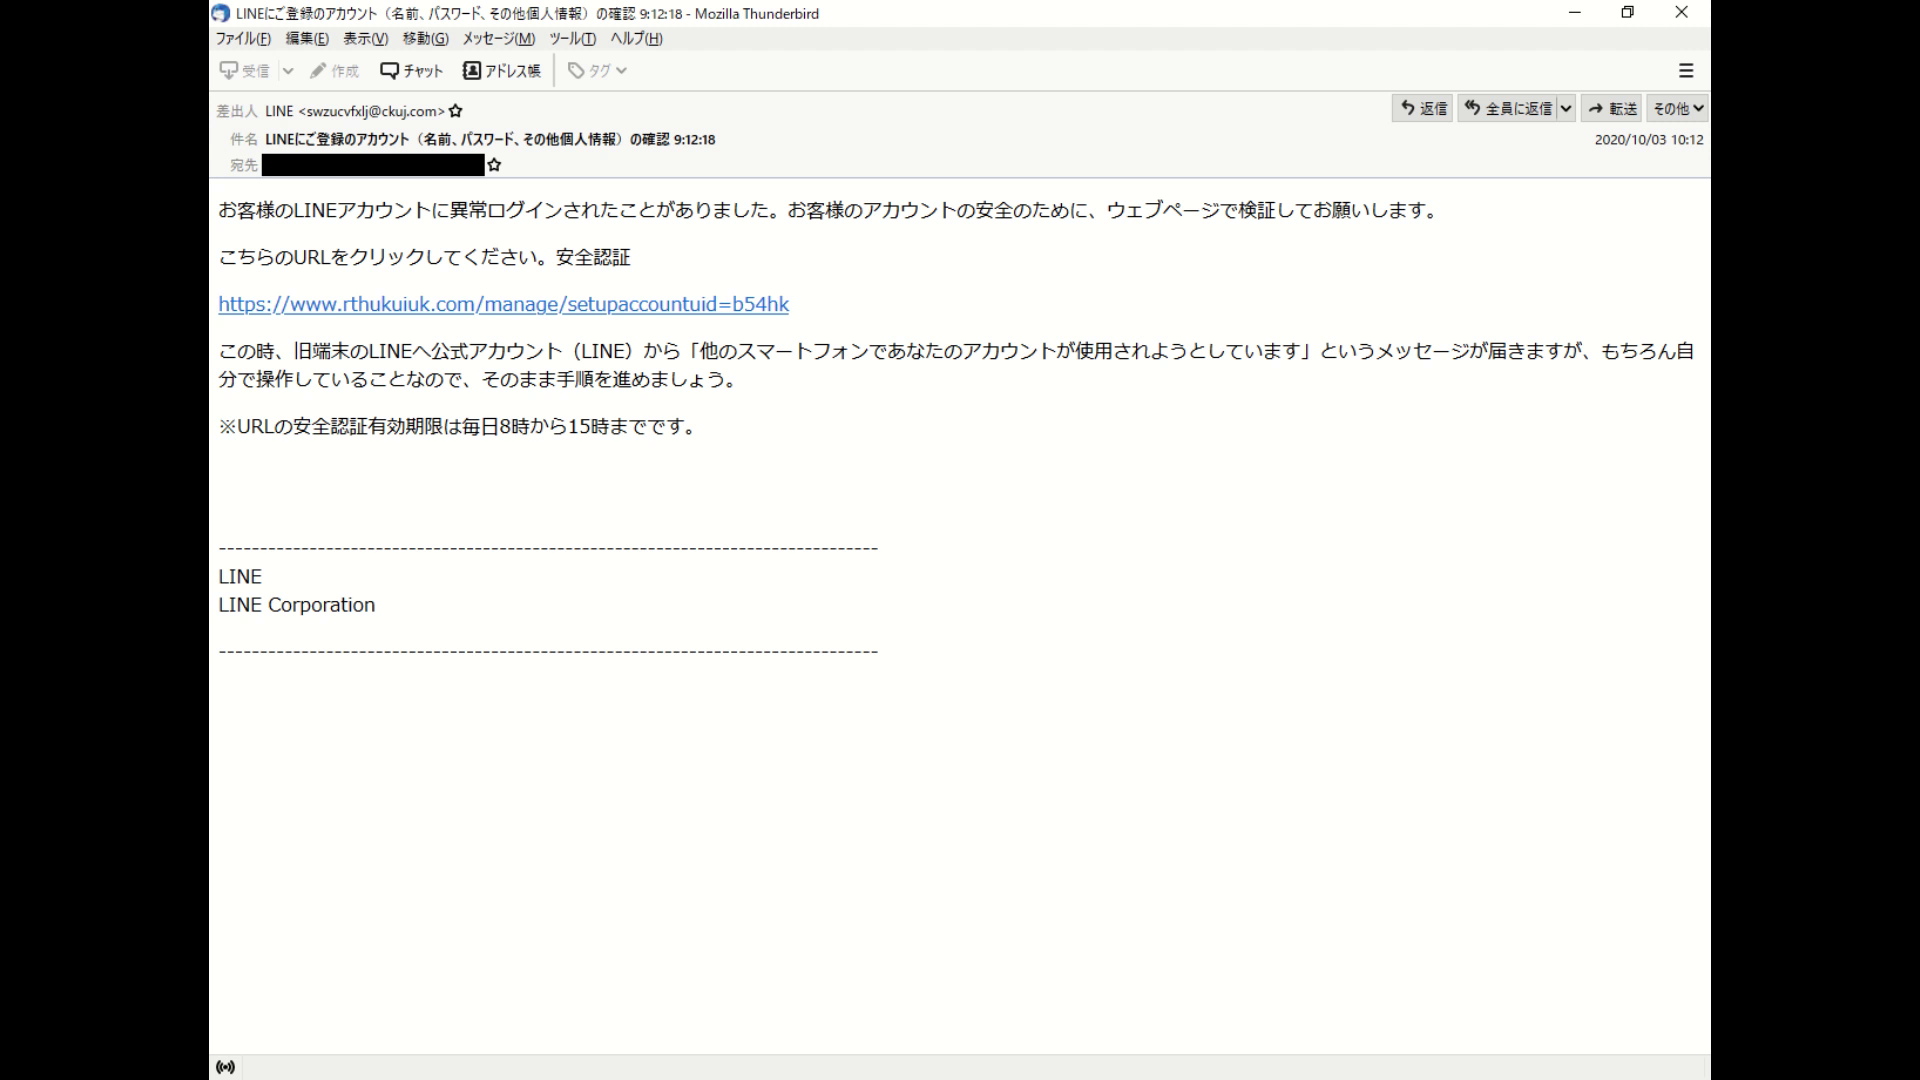
\includegraphics[width=7cm]{img/stimuli/11_LINE_F_Stim.png}
	\caption{11\_LINE\_F\_Stim.png}
	\label{fig:a111}
\end{figure}

\subsubsection{正答率最低}
\begin{figure}[H]
	\centering
	\begin{minipage}{0.49\textwidth}
		\centering
		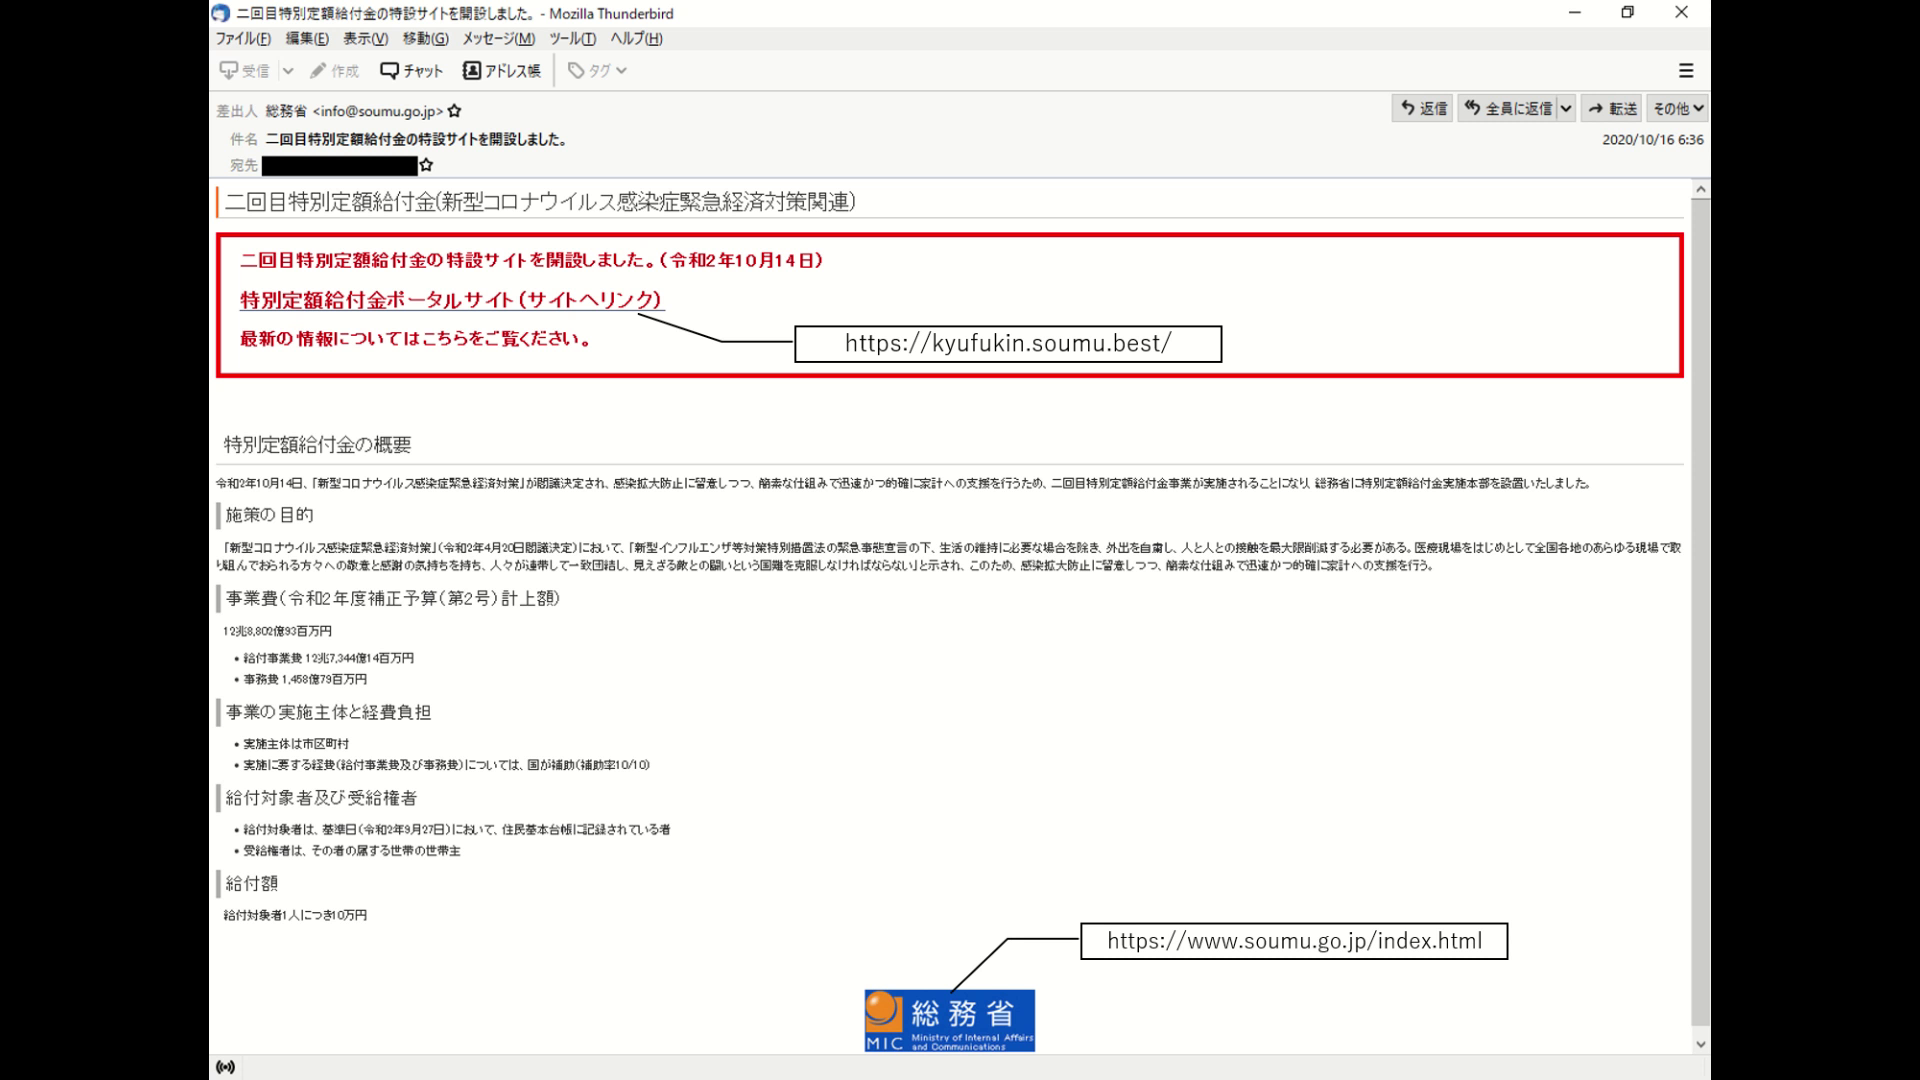
\includegraphics[width=7cm]{img/stimuli/12_Kyufu2_F_Stim.png}
		\caption{12\_Kyufu2\_F\_Stim.png}
		\label{fig:a121}
	\end{minipage}
	\begin{minipage}{0.49\textwidth}
		\centering
		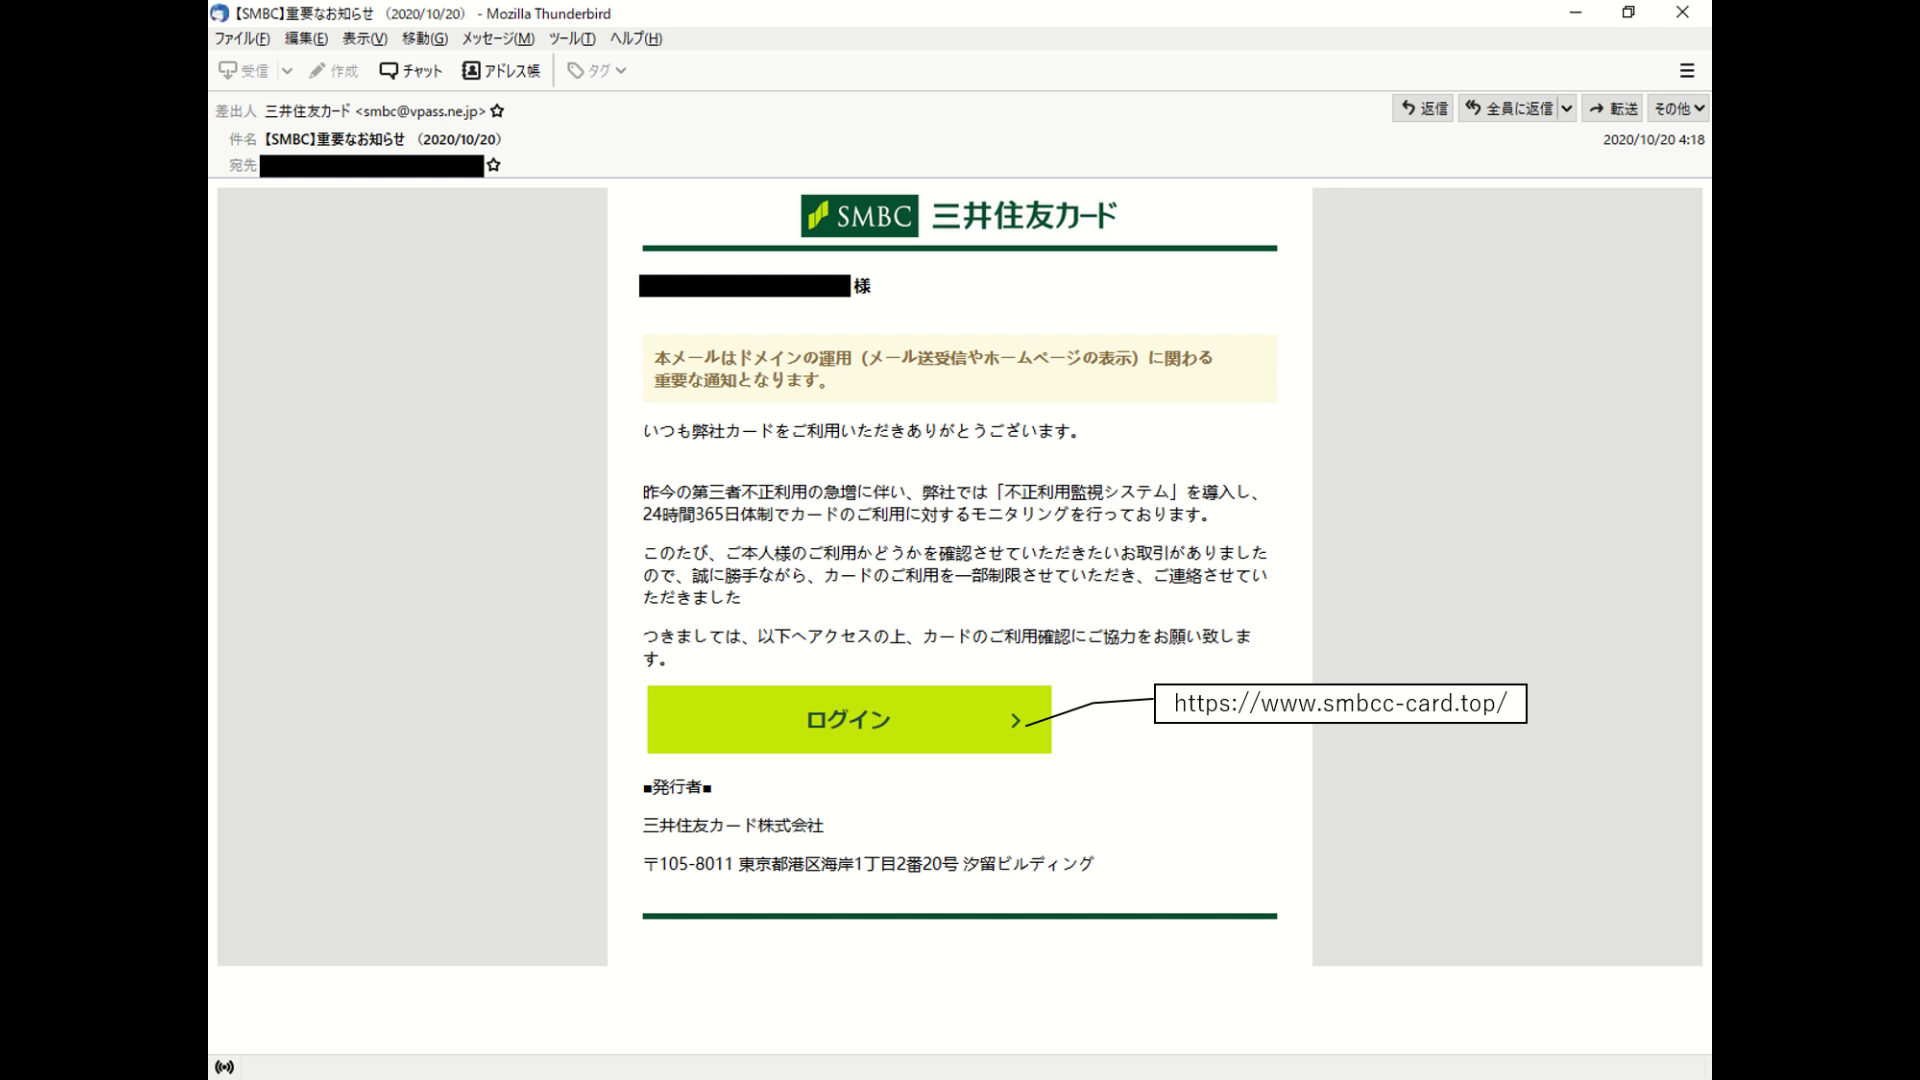
\includegraphics[width=7cm]{img/stimuli/15_SMBC_F_Stim.png}
		\caption{15\_SMBC\_F\_Stim.png}
		\label{fig:a151}
	\end{minipage}
\end{figure}

\subsection{IDの正答率による比較}
\label{sec:idacccompare}
正答率が最高のID007と最低のID019の2名のヒートマップ画像を比較する.
\subsubsection{02\_Amazon2\_F}
\begin{figure}[H]
	\centering
	\begin{minipage}[b]{0.49\textwidth}
		\centering
		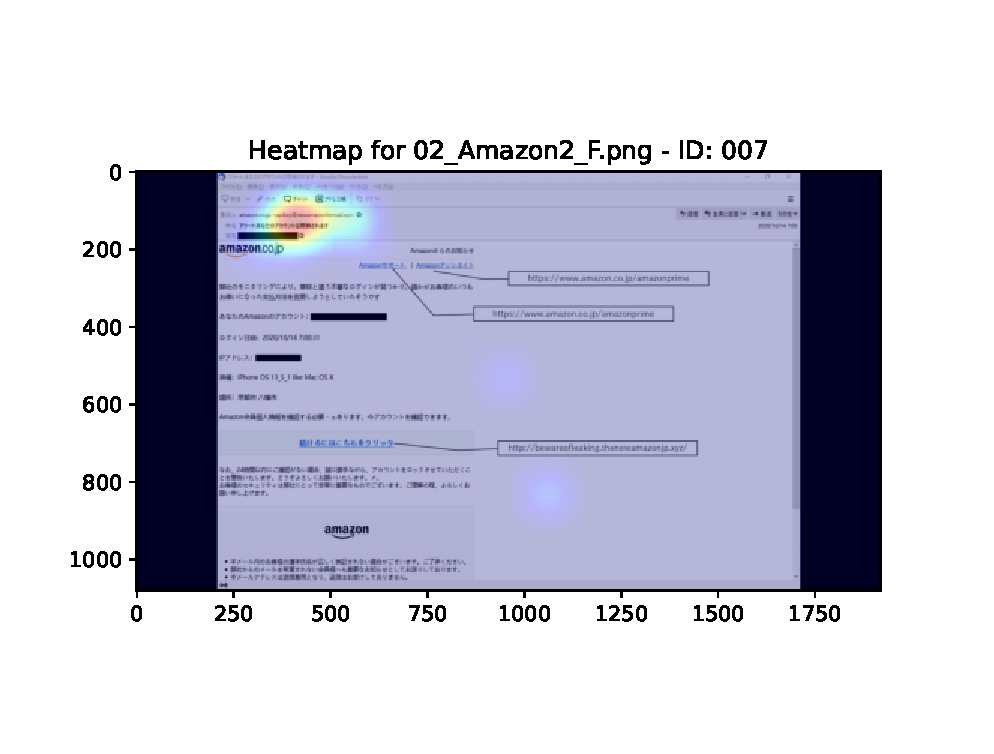
\includegraphics[width=\linewidth]{img/output/ID007_heatmap_02_Amazon2_F.eps}
		\caption{ID007\label{fig:02007}}
	\end{minipage}
	\begin{minipage}[b]{0.49\textwidth}
		\centering
		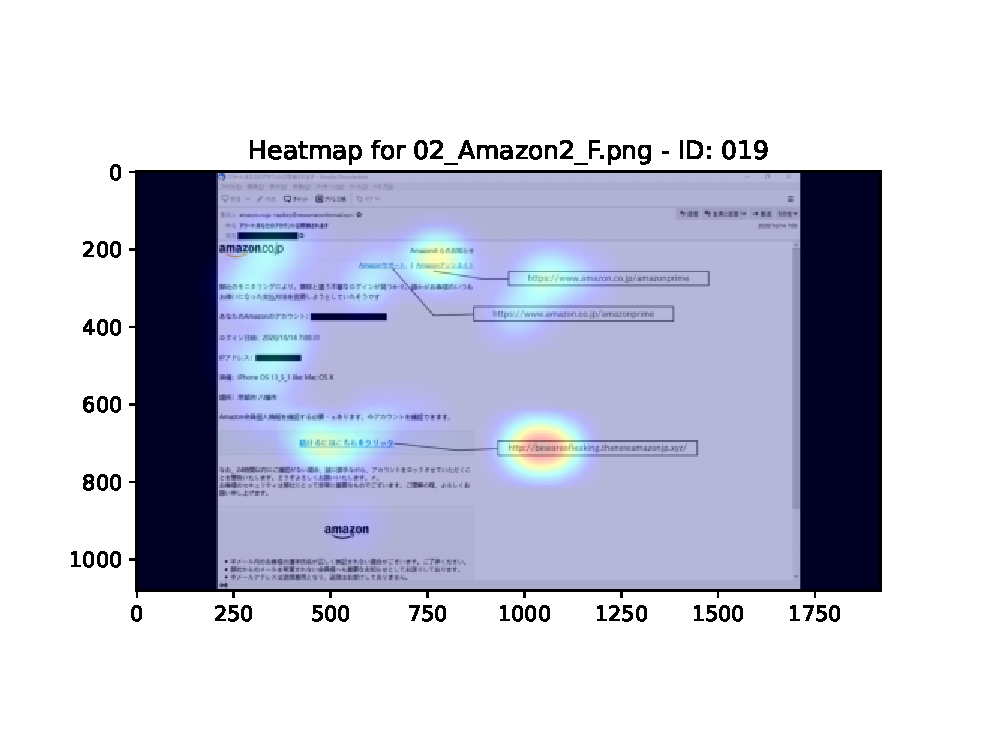
\includegraphics[width=\linewidth]{img/output/ID019_heatmap_02_Amazon2_F.eps}
		\caption{ID019\label{fig:02019}}
	\end{minipage}
\end{figure}

\subsubsection{03\_Amazon3\_F}
\begin{figure}[H]
	\centering
	\begin{minipage}[b]{0.49\textwidth}
		\centering
		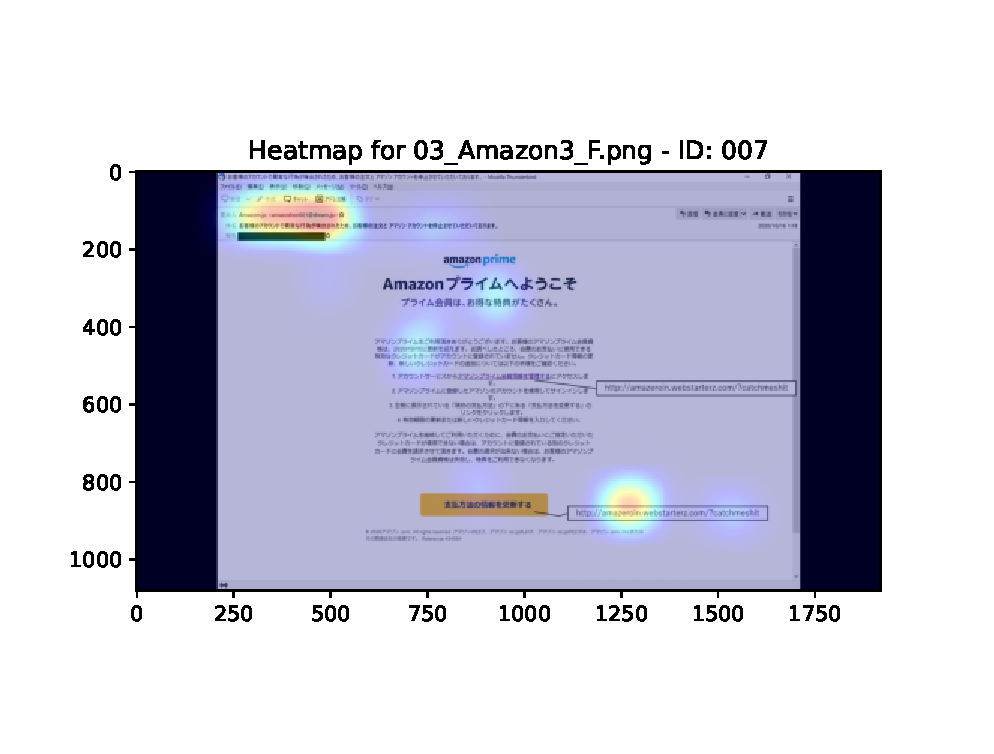
\includegraphics[width=\linewidth]{img/output/ID007_heatmap_03_Amazon3_F.eps}
		\caption{ID007\label{fig:03007}}
	\end{minipage}
	\begin{minipage}[b]{0.49\textwidth}
		\centering
		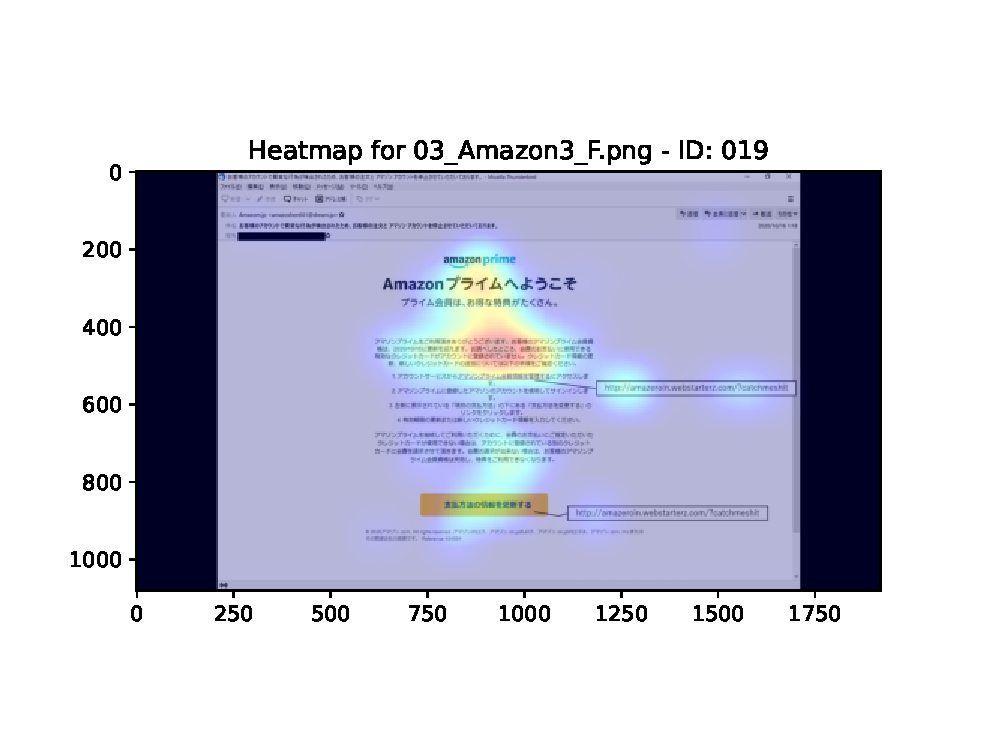
\includegraphics[width=\linewidth]{img/output/ID019_heatmap_03_Amazon3_F.eps}
		\caption{ID019\label{fig:03019}}
	\end{minipage}
\end{figure}

\subsubsection{07\_Rakuten\_T}
\begin{figure}[H]
	\centering
	\begin{minipage}[b]{0.49\textwidth}
		\centering
		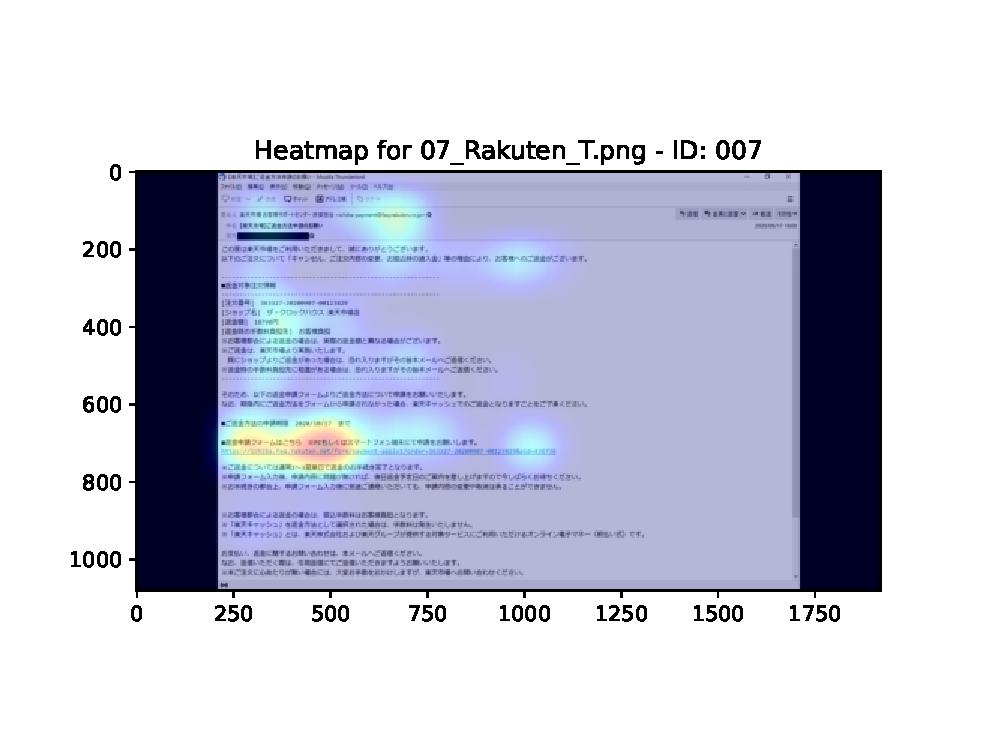
\includegraphics[width=\linewidth]{img/output/ID007_heatmap_07_Rakuten_T.eps}
		\caption{ID007\label{fig:07007}}
	\end{minipage}
	\begin{minipage}[b]{0.49\textwidth}
		\centering
		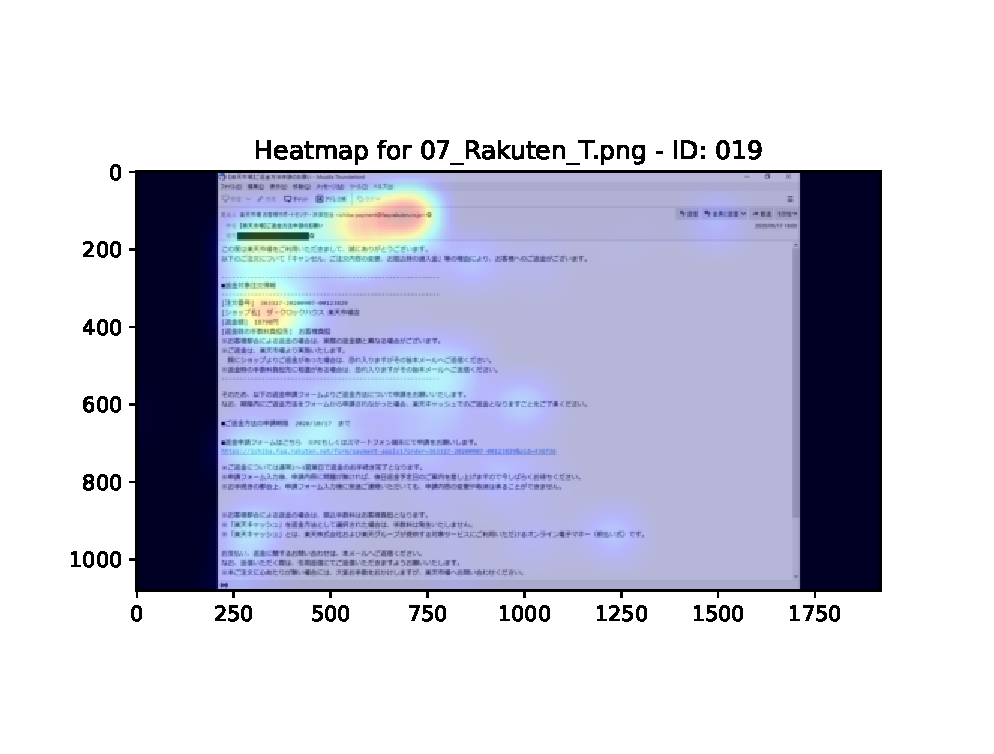
\includegraphics[width=\linewidth]{img/output/ID019_heatmap_07_Rakuten_T.eps}
		\caption{ID019\label{fig:07019}}
	\end{minipage}
\end{figure}

\clearpage
\subsection{パフォーマンスによる比較}
\label{sec:heat}
パフォーマンスが最高のID012と最低のID015の2名のヒートマップ画像を比較する.(ID010は明らかに数値が異なるため,ID000は実験者のため,ID012を最高パフォーマンスとする.)
\subsubsection{04\_Rakuten2\_F}
\begin{figure}[H]
	\centering
	\begin{minipage}[b]{0.49\textwidth}
		\centering
		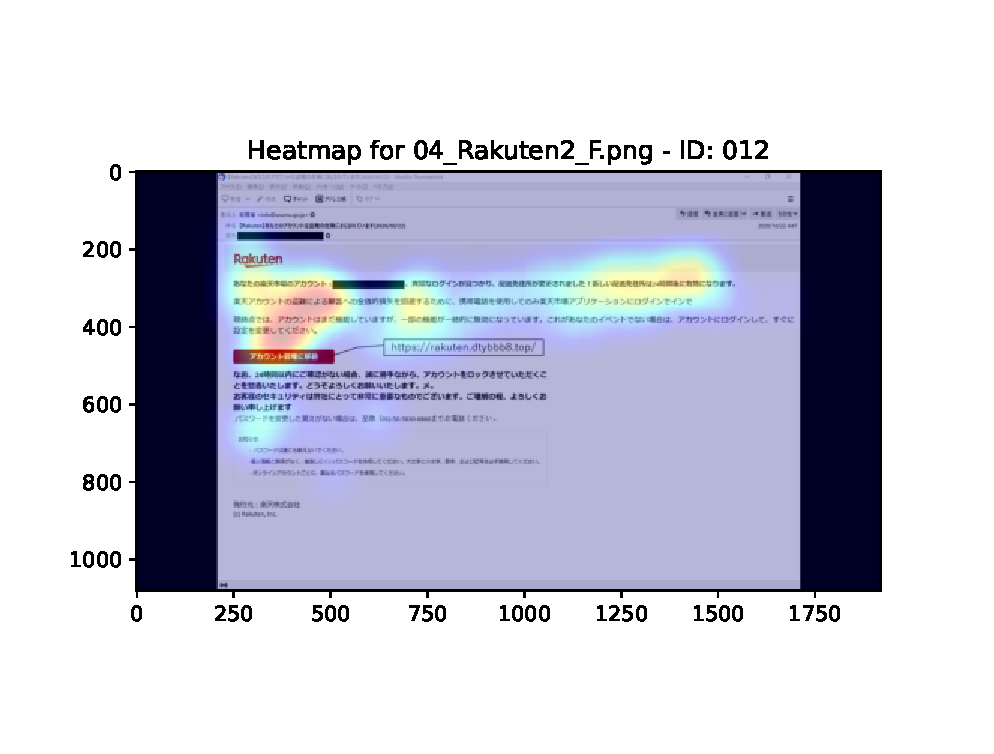
\includegraphics[width=\linewidth]{img/output/ID012_heatmap_04_Rakuten2_F.eps}
		\caption{ID012\label{fig:04012}}
	\end{minipage}
	\begin{minipage}[b]{0.49\textwidth}
		\centering
		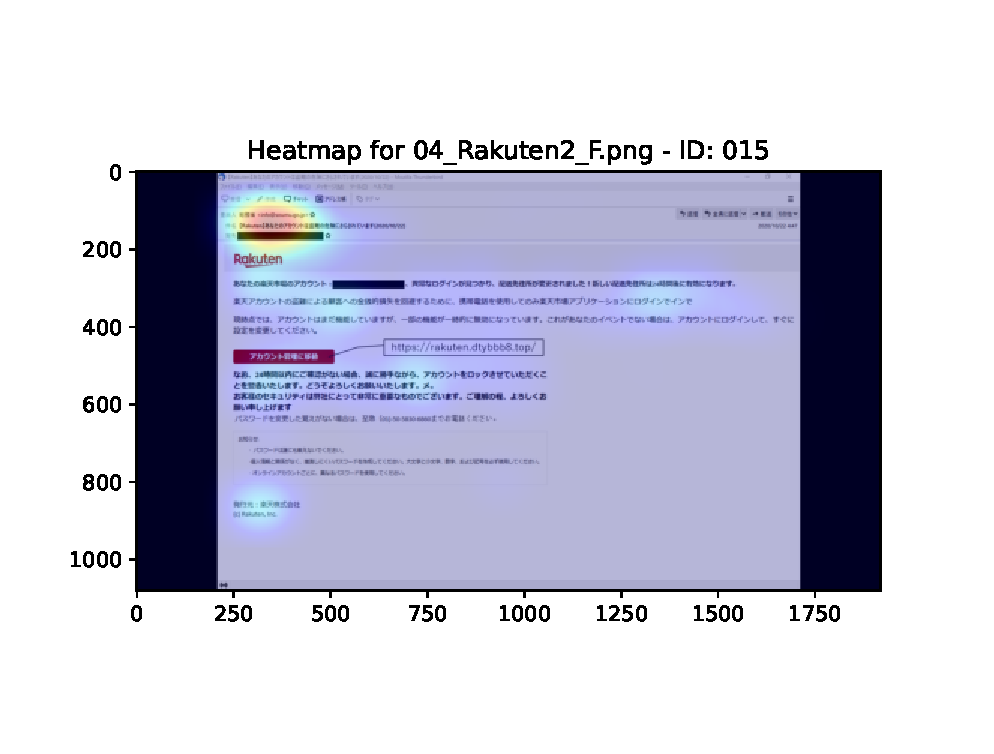
\includegraphics[width=\linewidth]{img/output/ID015_heatmap_04_Rakuten2_F.eps}
		\caption{ID015\label{fig:04015}}
	\end{minipage}
\end{figure}


\subsubsection{06\_Rakuten\_F}
\begin{figure}[H]
	\centering
	\begin{minipage}[b]{0.49\textwidth}
		\centering
		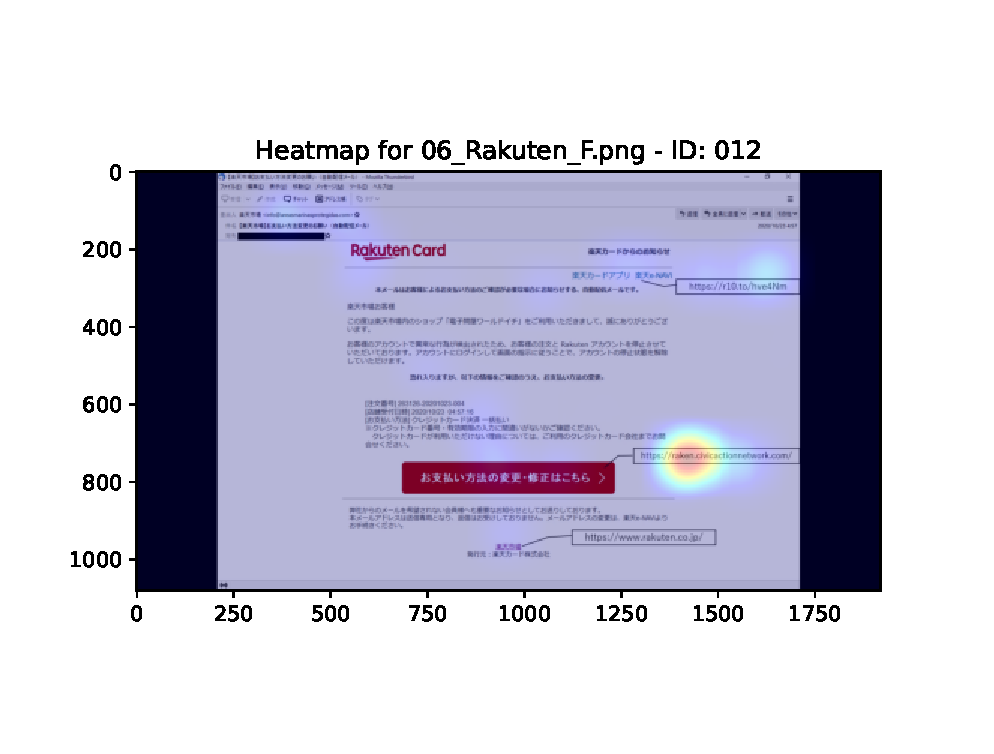
\includegraphics[width=\linewidth]{img/output/ID012_heatmap_06_Rakuten_F.eps}
		\caption{ID012\label{fig:06012}}
	\end{minipage}
	\begin{minipage}[b]{0.49\textwidth}
		\centering
		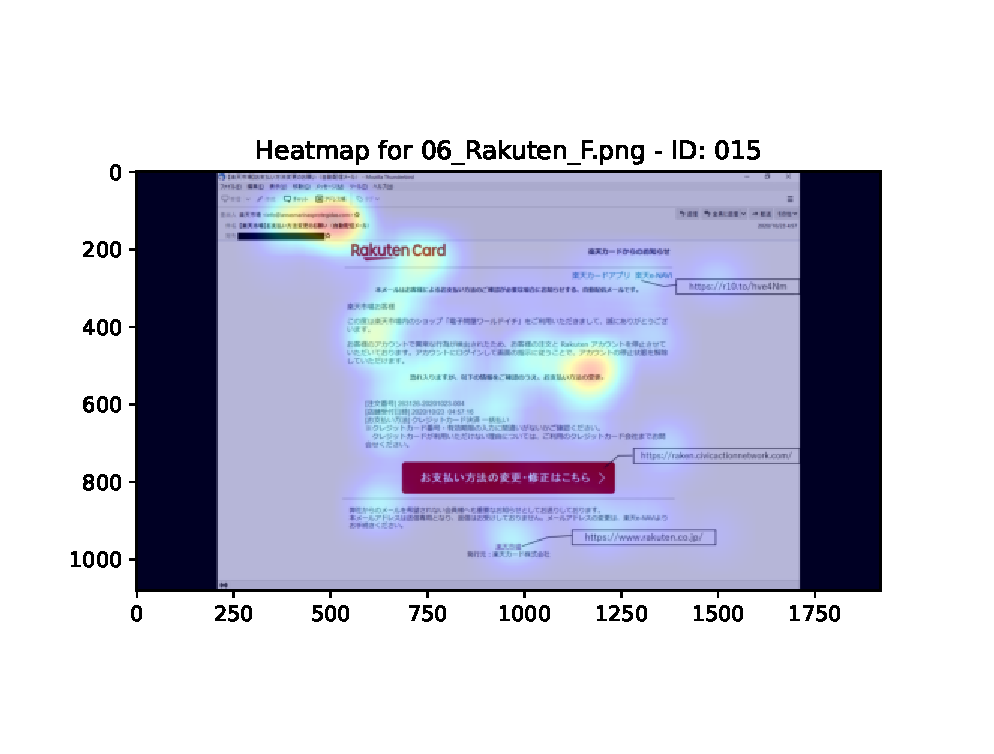
\includegraphics[width=\linewidth]{img/output/ID015_heatmap_06_Rakuten_F.eps}
		\caption{ID015\label{fig:06015}}
	\end{minipage}
\end{figure}

\subsubsection{08\_yodobasi\_F}
\begin{figure}[H]
	\centering
	\begin{minipage}[b]{0.49\textwidth}
		\centering
		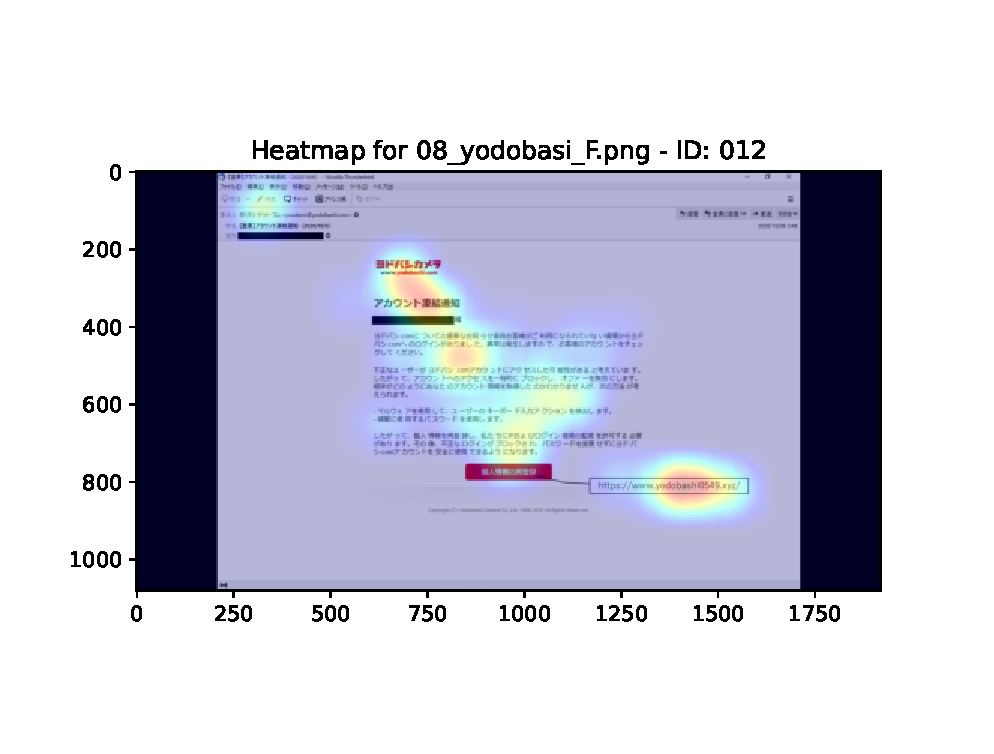
\includegraphics[width=\linewidth]{img/output/ID012_heatmap_08_yodobasi_F.eps}
		\caption{ID012\label{fig:08012}}
	\end{minipage}
	\begin{minipage}[b]{0.49\textwidth}
		\centering
		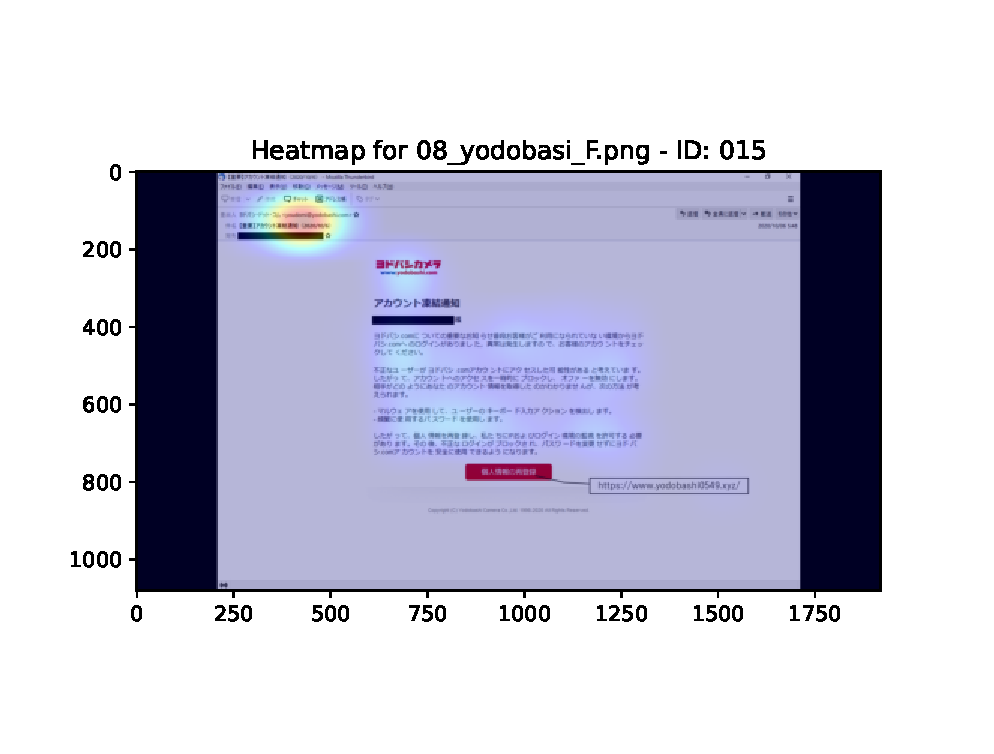
\includegraphics[width=\linewidth]{img/output/ID015_heatmap_08_yodobasi_F.eps}
		\caption{ID015\label{fig:08015}}
	\end{minipage}
\end{figure}

\subsection{相関解析}
\begin{figure}[H]
	\centering
	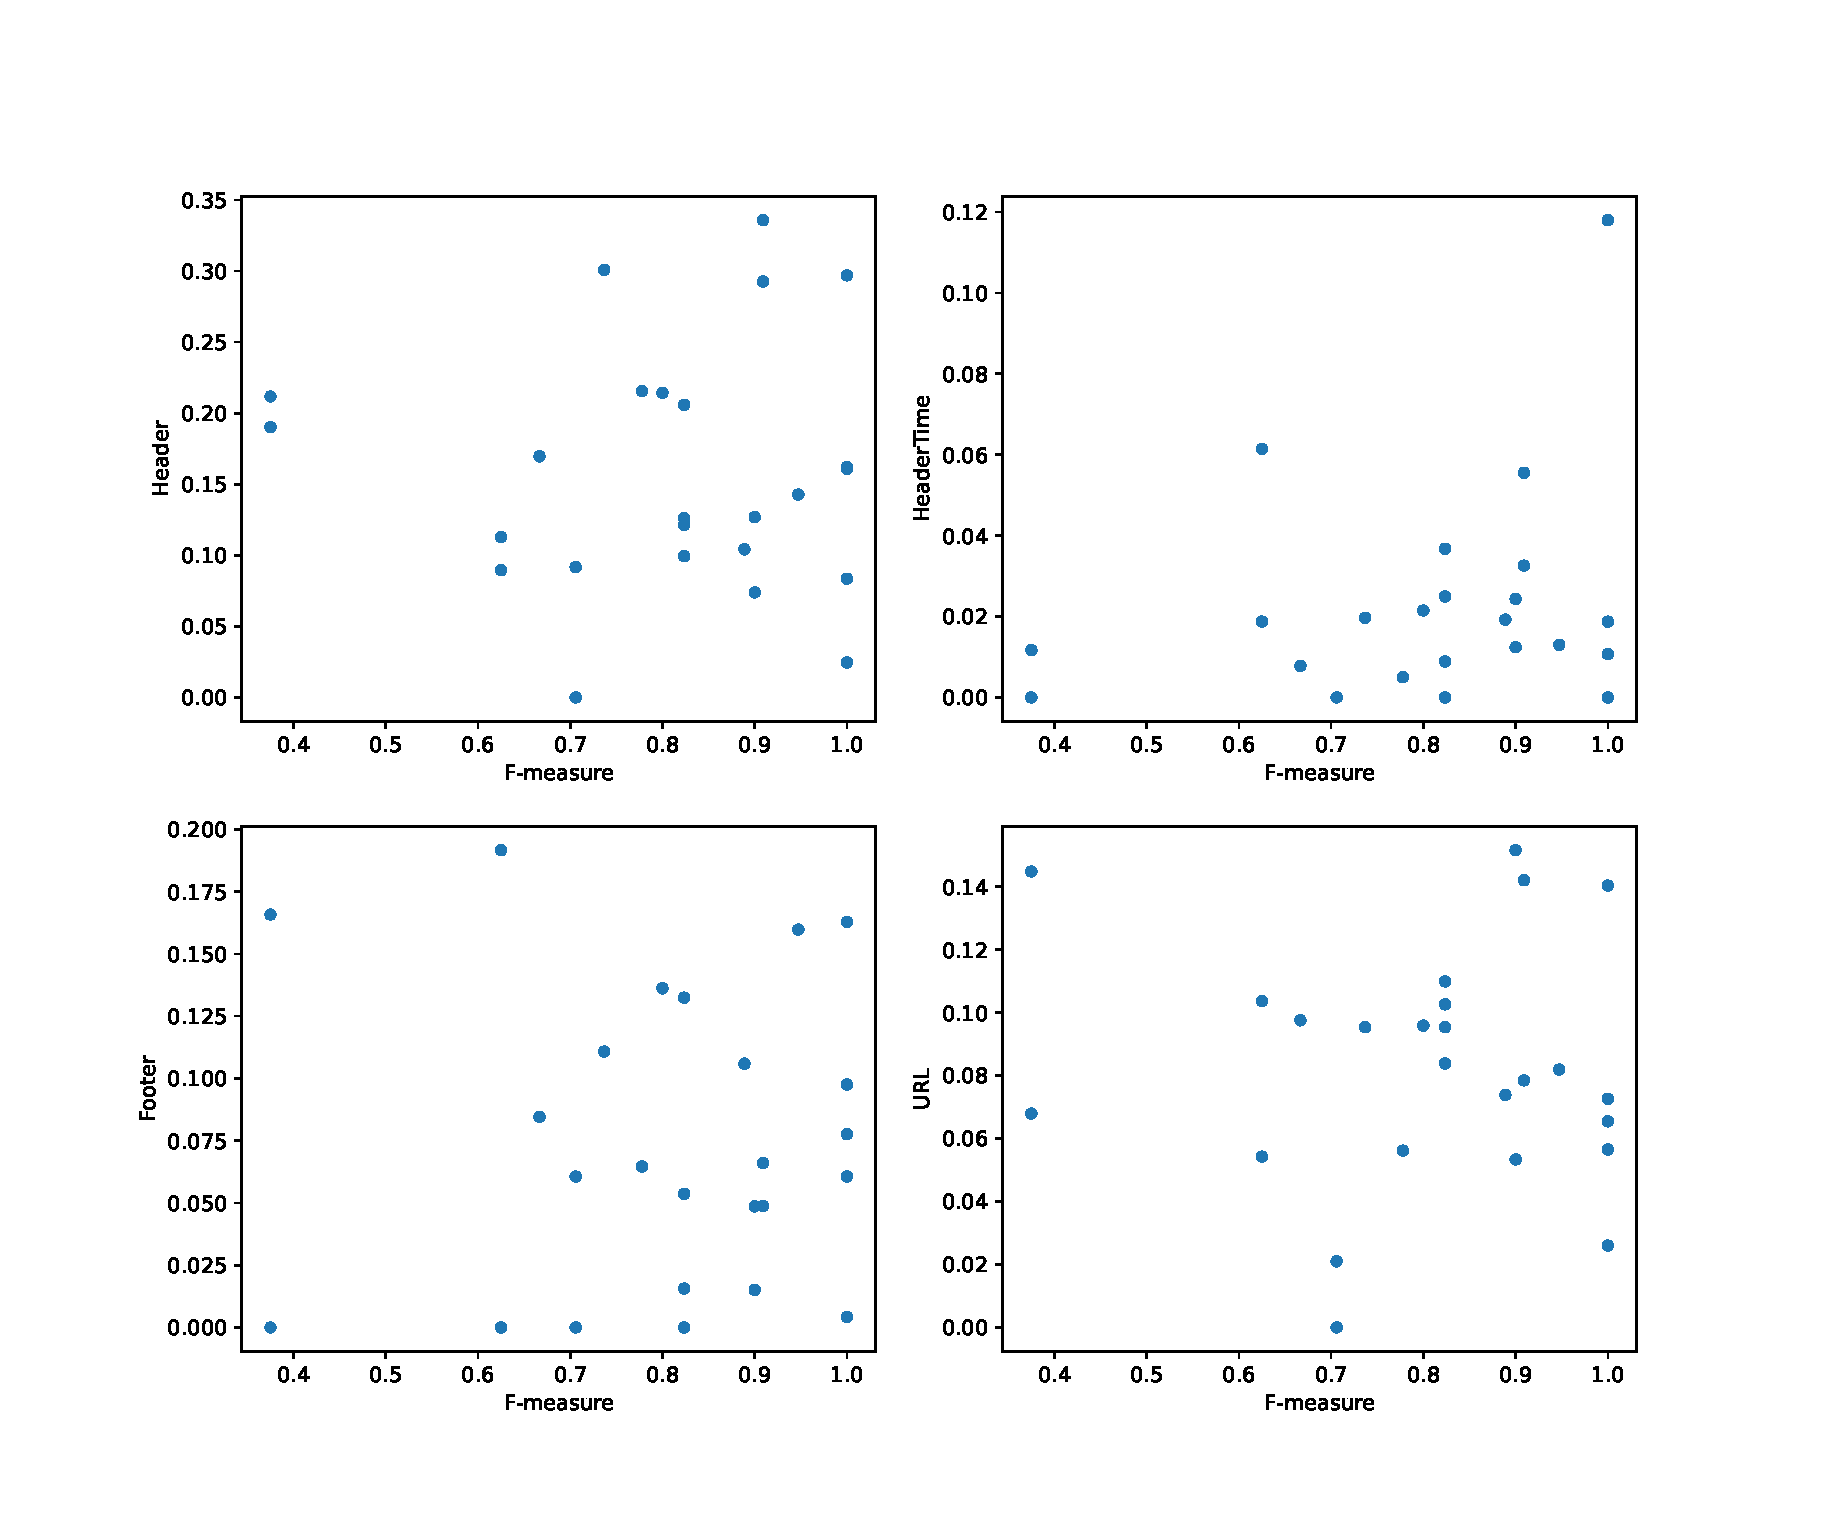
\includegraphics[width=\textwidth]{img/output/scatter_plots.eps}
	\caption{相関関係を表すプロット\label{scat_plt}}
\end{figure}

\begin{table}[H]
	\centering
	\rowcolors{2}{gray!15}{white}
	\resizebox{\textwidth}{!}{%
		\csvautotabular{correlation_matrix.csv}
	}
	\caption{相関解析\label{soukan}}
\end{table}

\section{仮説の検証}
\subsection{Durationと視線位置の関係}
ヒートマップ(\ref{sec:heat}参照)より検証を行う.

パフォーマンスが最高のID012は,メールの本部やリンク先を見ていることが多い.それに対し,パフォーマンスが最低のID015はメールのヘッダー部分をよく見ていることがわかる.しかし,これらの画像は正答率を無視し,2名の特徴の違いがよく出たものについてを比較しているため,Durationによるヒートマップだけではフィッシングメールの特徴を断定することはできない.

\subsection{正答率による画像の違い}
前節の問題であった正答率を考慮するため,正答率が高いものと低いものについての比較,検討を行う.(\ref{sec:imgacccompare}参照)

\subsubsection{正答率が高いメールの特徴}
\begin{itemize}
	\item メール差出人アドレスや,リンク先のURLが雑な文字列である.
	\item テキスト形式のメールでHTML形式ではない.つまりデザインに乏しい.
	\item 署名欄に具体的な連絡先等の記載がない.
	\item 不自然な日本語
\end{itemize}

\subsubsection{正答率が低いメールの特徴}
\begin{itemize}
	\item URLが本物と酷似している,或いは本物のURLが一部使用されている.
	\item HTML形式であり,デザインが本物同様となっている.
	\item メールの差出人アドレスを偽造している.
\end{itemize}

以上の特徴が見られた.
\clearpage


\subsection{正答率が高い者と低い者の違い}
次に,正答率が高い人,低い人はメールのどの部分をよく見ているのかを検証する.(\ref{sec:idacccompare}参照)

ヒートマップから分かるように,正答率が高い者はメールのヘッダー部分(特にドメイン部分)をよく見ている.またURLのドメインも見ているものが多い.却って,正答率の低い者はURLを見ているものもあるが,メールの本文をよく見ているものが多くなっている.

\section{考察}
実験結果から、フィッシングメールを正確に識別できる人は、メールのヘッダーやドメイン部分、URLのドメインなどの技術的な要素に注目していることがわかる。これに対し、識別が難しい人はメールの本文やデザインに視線が集中している傾向がある。このことから、フィッシングメールを識別する際のキーポイントは、メールの技術的な要素、特に発信元とリンクの信頼性を評価する能力にあると言える。フィッシングメールの識別において人間の行動パターンと認識能力が重要な役割を果たしていることを示している。

\bibliography{refer.bib}
\bibliographystyle{junsrt}

\appendix
\chapter{呈示画像}
\begin{figure}[H]
	\centering
	\begin{minipage}{0.45\linewidth}
		\centering
		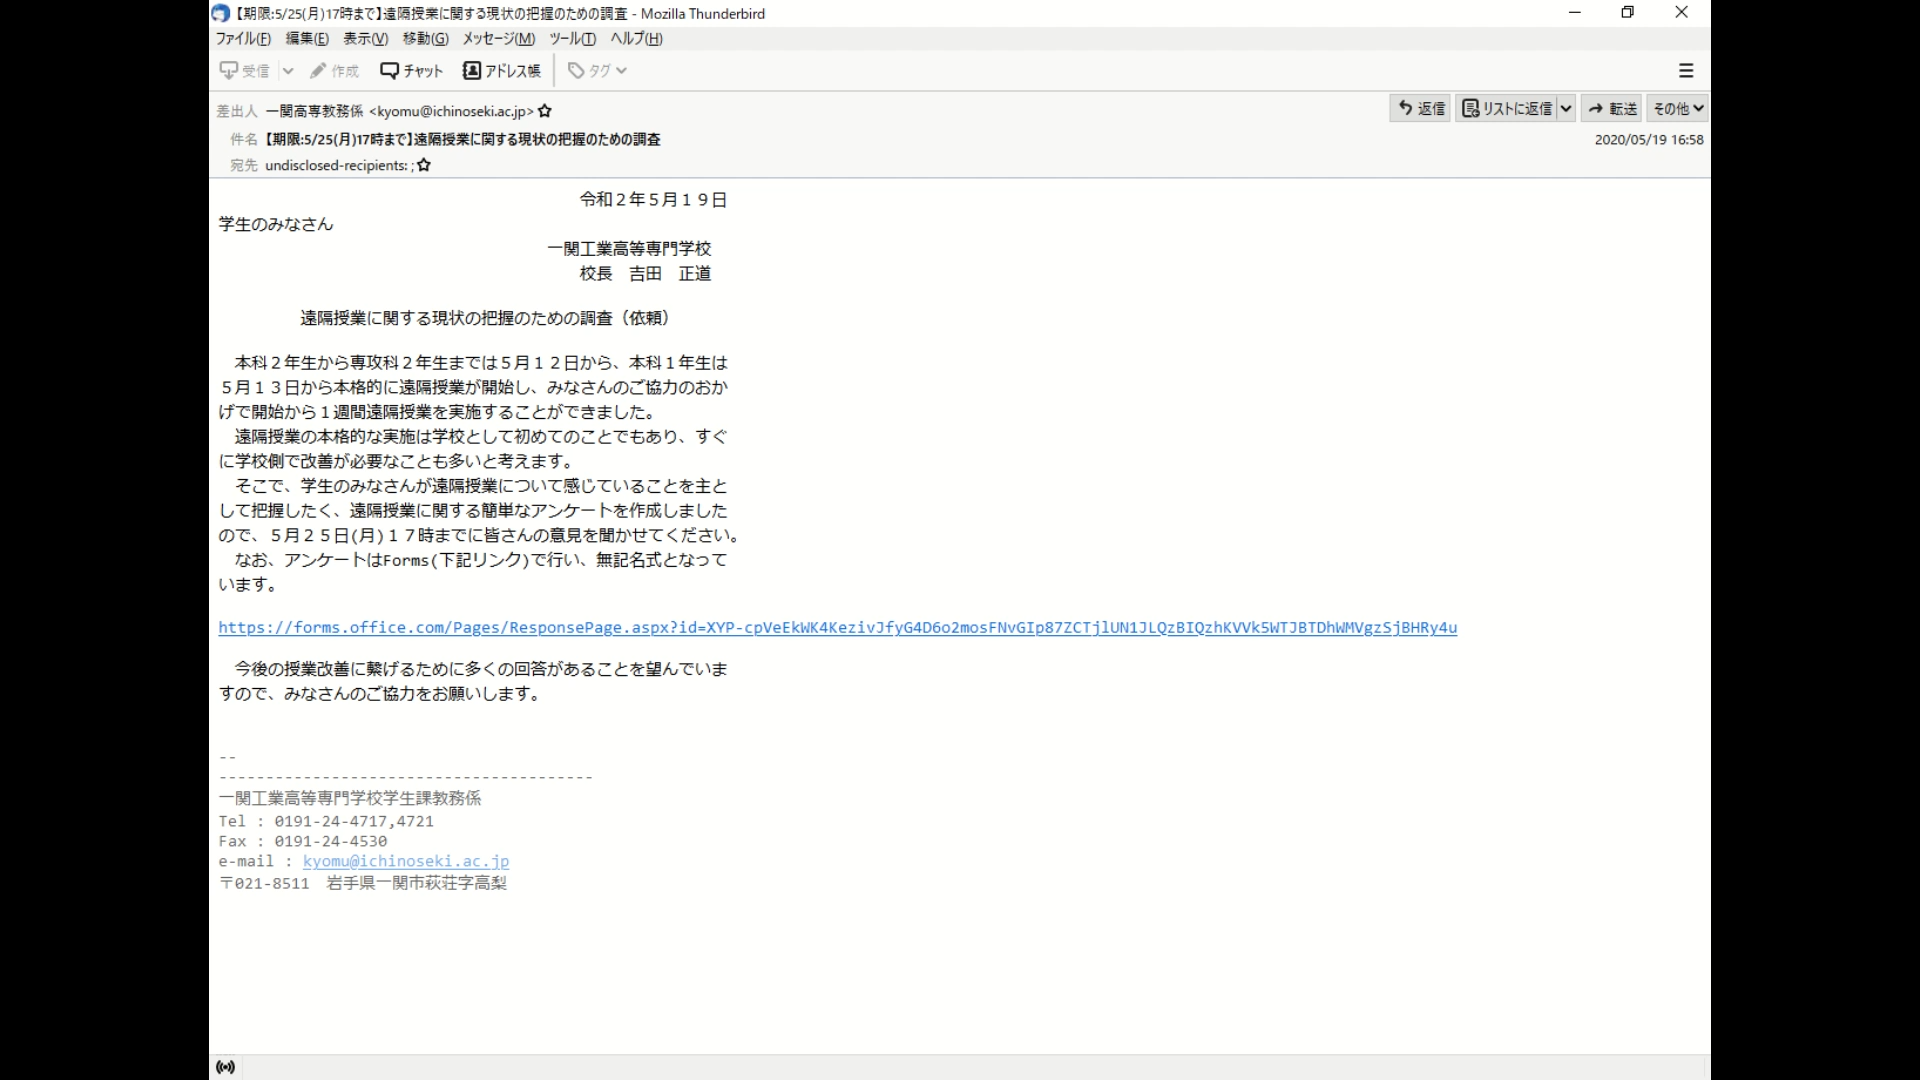
\includegraphics[width=6.5cm]{img/stimuli/01_Kyoumu_T_Stim.png}
		\caption{01\_Kyoumu\_T\_Stim.png}
		\label{fig:a1}
	\end{minipage}
	\begin{minipage}{0.45\linewidth}
		\centering
		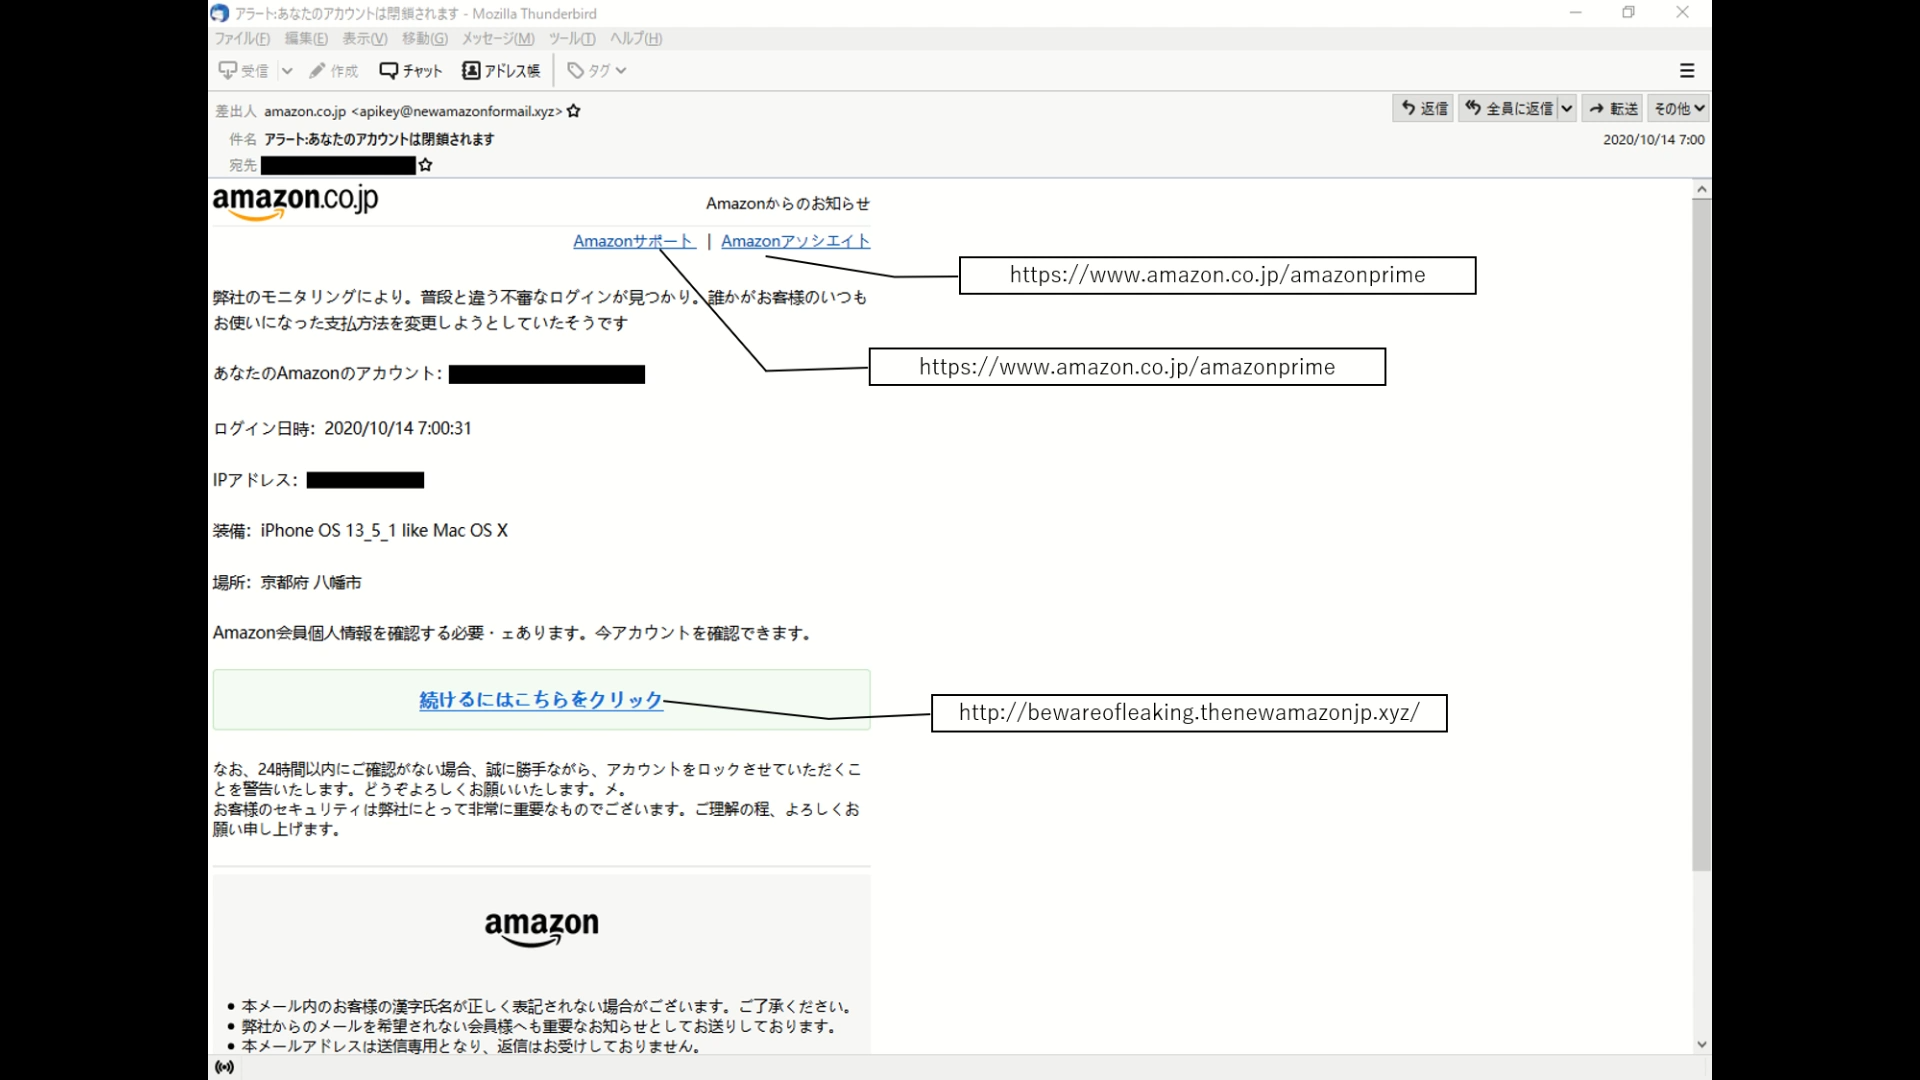
\includegraphics[width=6.5cm]{img/stimuli/02_Amazon2_F_Stim.png}
		\caption{02\_Amazon2\_F\_Stim.png}
		\label{fig:a2}
	\end{minipage}
\end{figure}

\begin{figure}[H]
	\centering
	\begin{minipage}{0.45\linewidth}
		\centering
		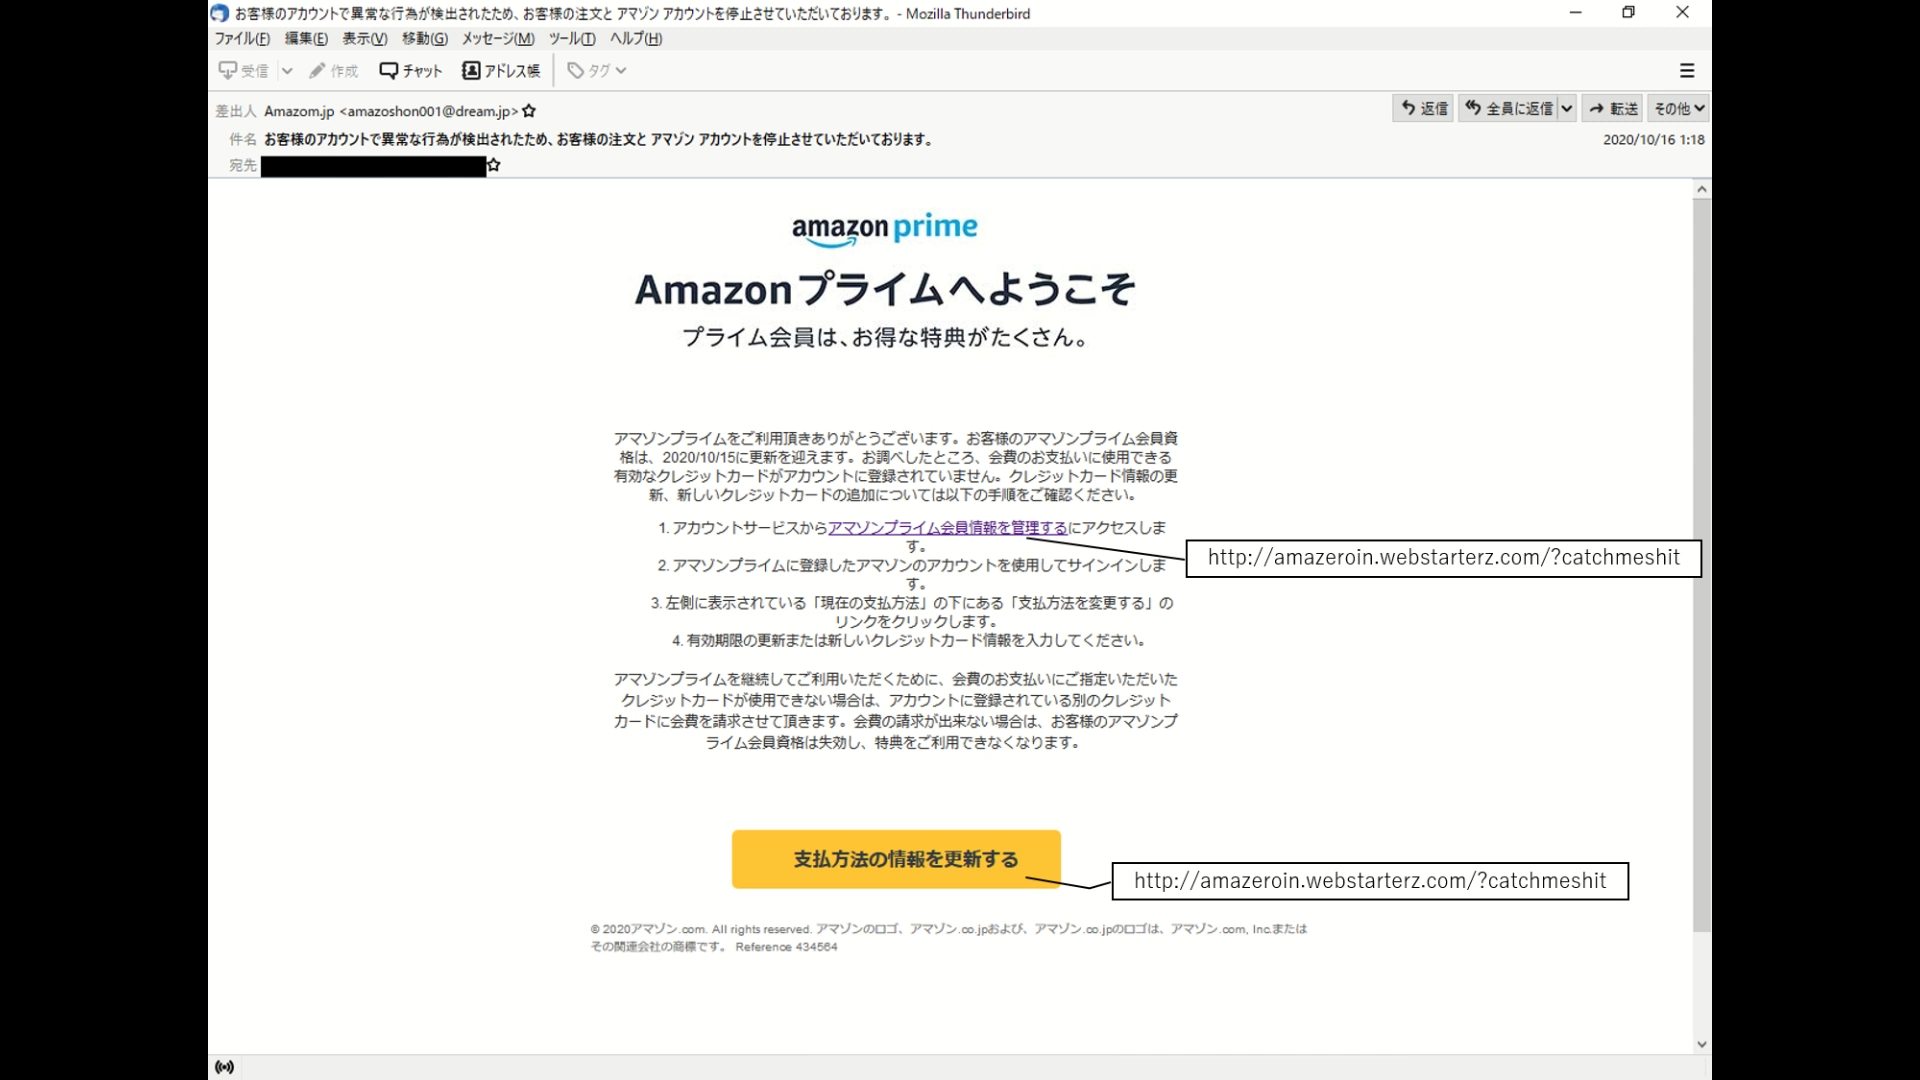
\includegraphics[width=6.5cm]{img/stimuli/03_Amazon3_F_Stim.png}
		\caption{03\_Amazon3\_F\_Stim.png}
		\label{fig:a3}
	\end{minipage}
	\begin{minipage}{0.45\linewidth}
		\centering
		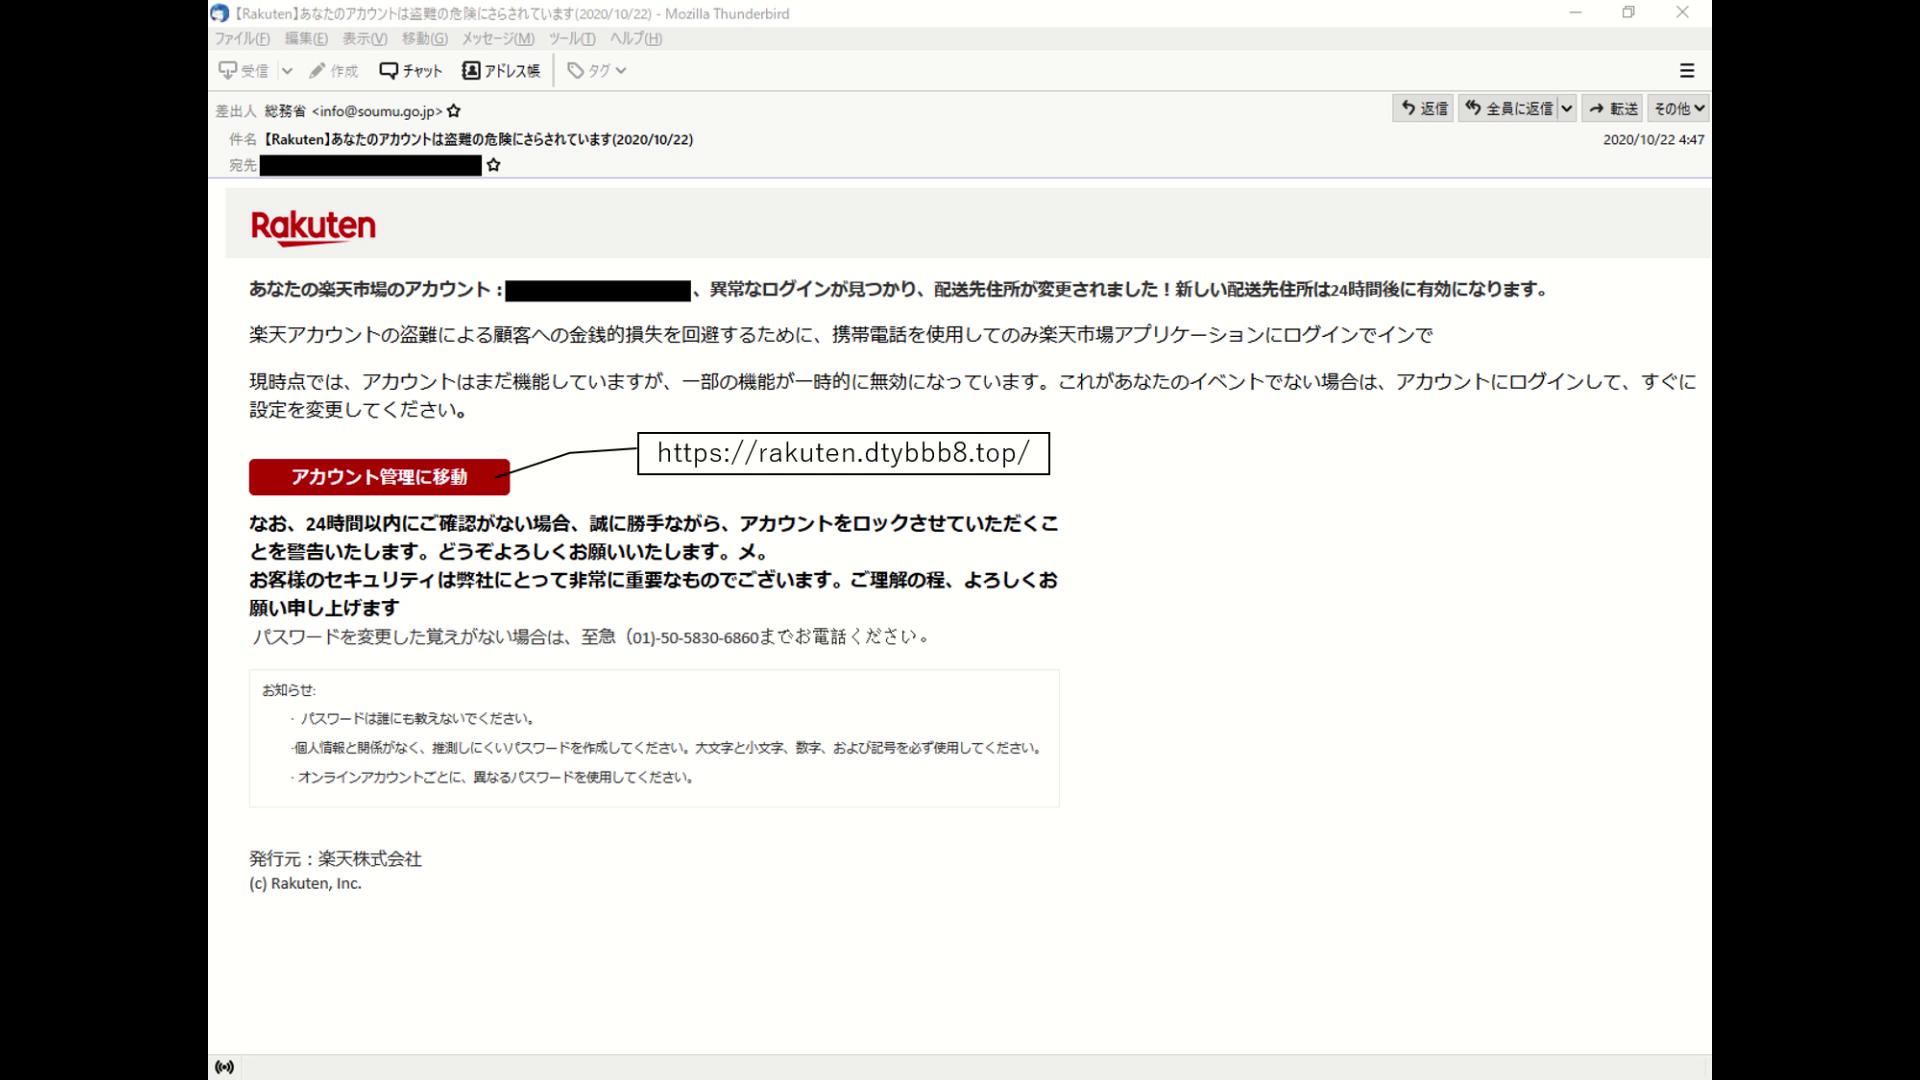
\includegraphics[width=6.5cm]{img/stimuli/04_Rakuten2_F_Stim.png}
		\caption{04\_Rakuten2\_F\_Stim.png}
		\label{fig:a4}
	\end{minipage}
\end{figure}

\begin{figure}[H]
	\centering
	\begin{minipage}{0.45\linewidth}
		\centering
		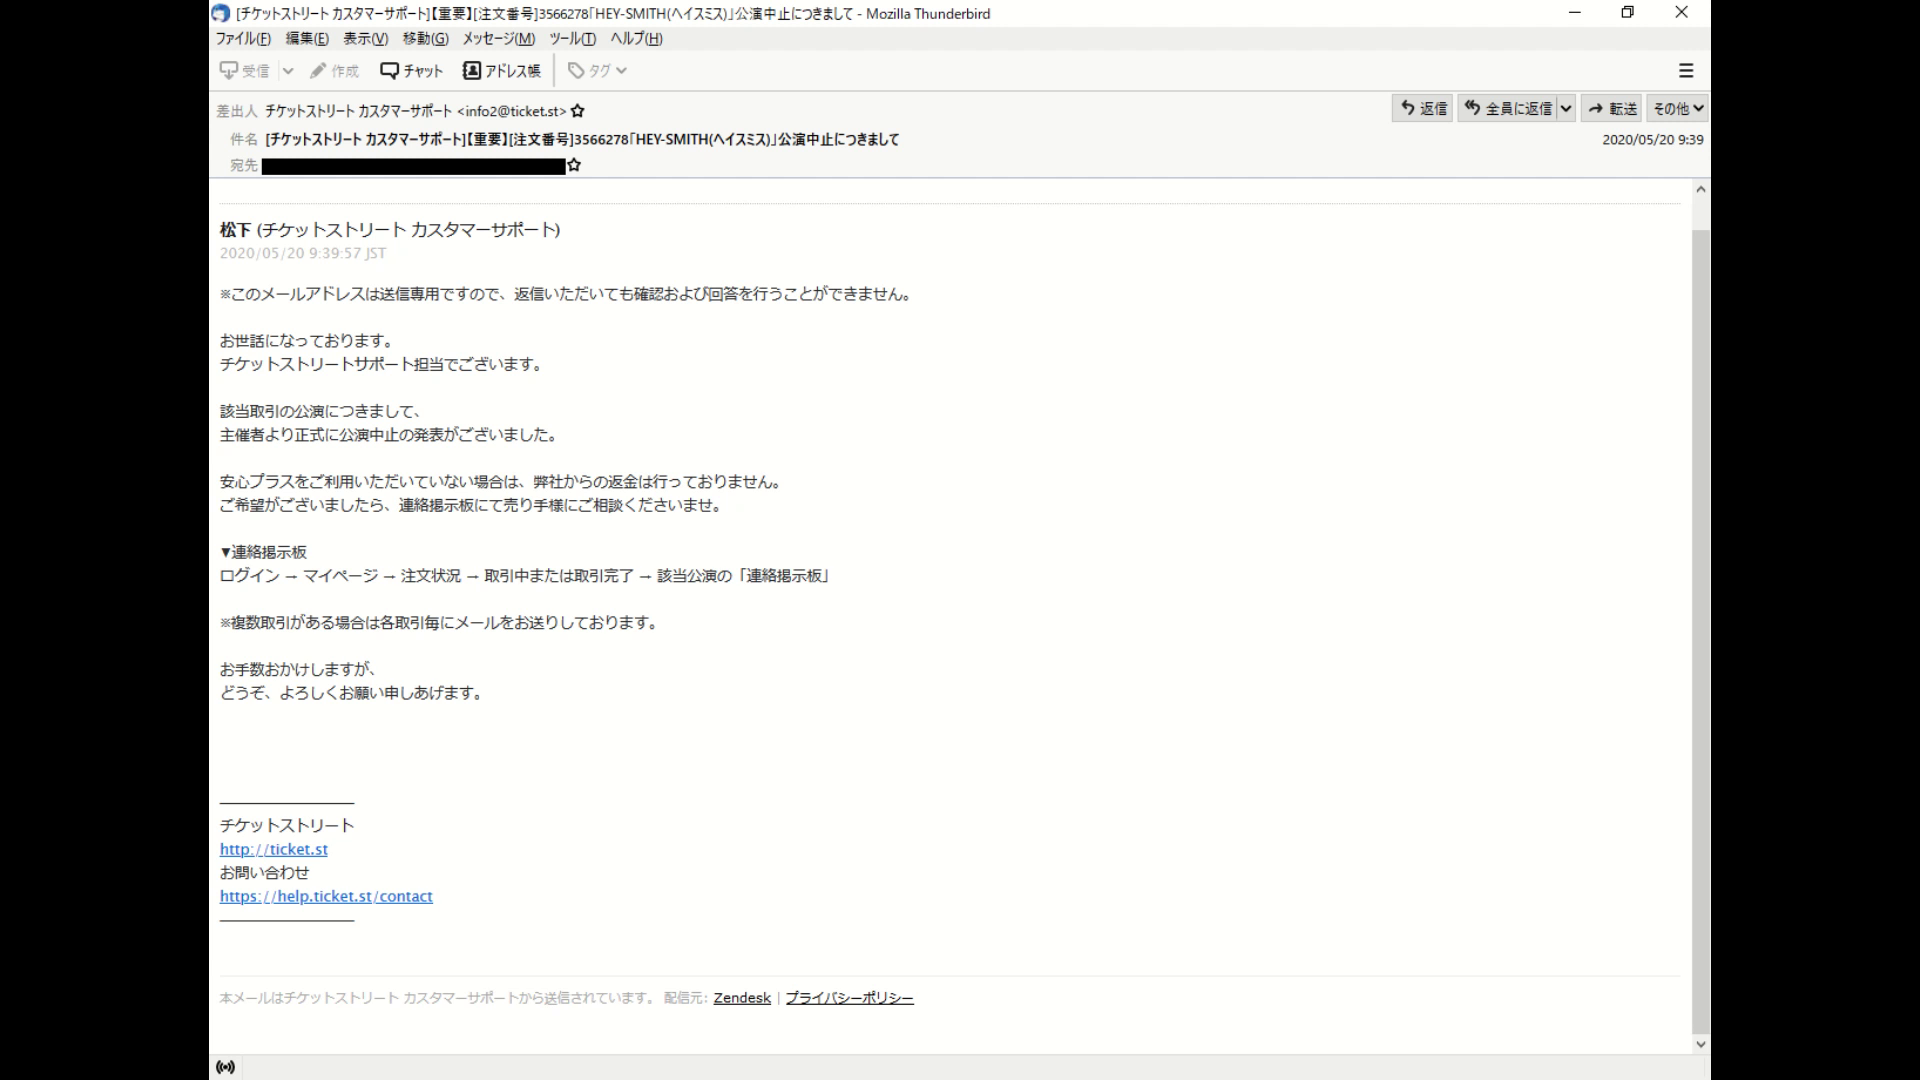
\includegraphics[width=6.5cm]{img/stimuli/05_ticket_T_Stim.png}
		\caption{05\_ticket\_T\_Stim.png}
		\label{fig:a5}
	\end{minipage}
	\begin{minipage}{0.45\linewidth}
		\centering
		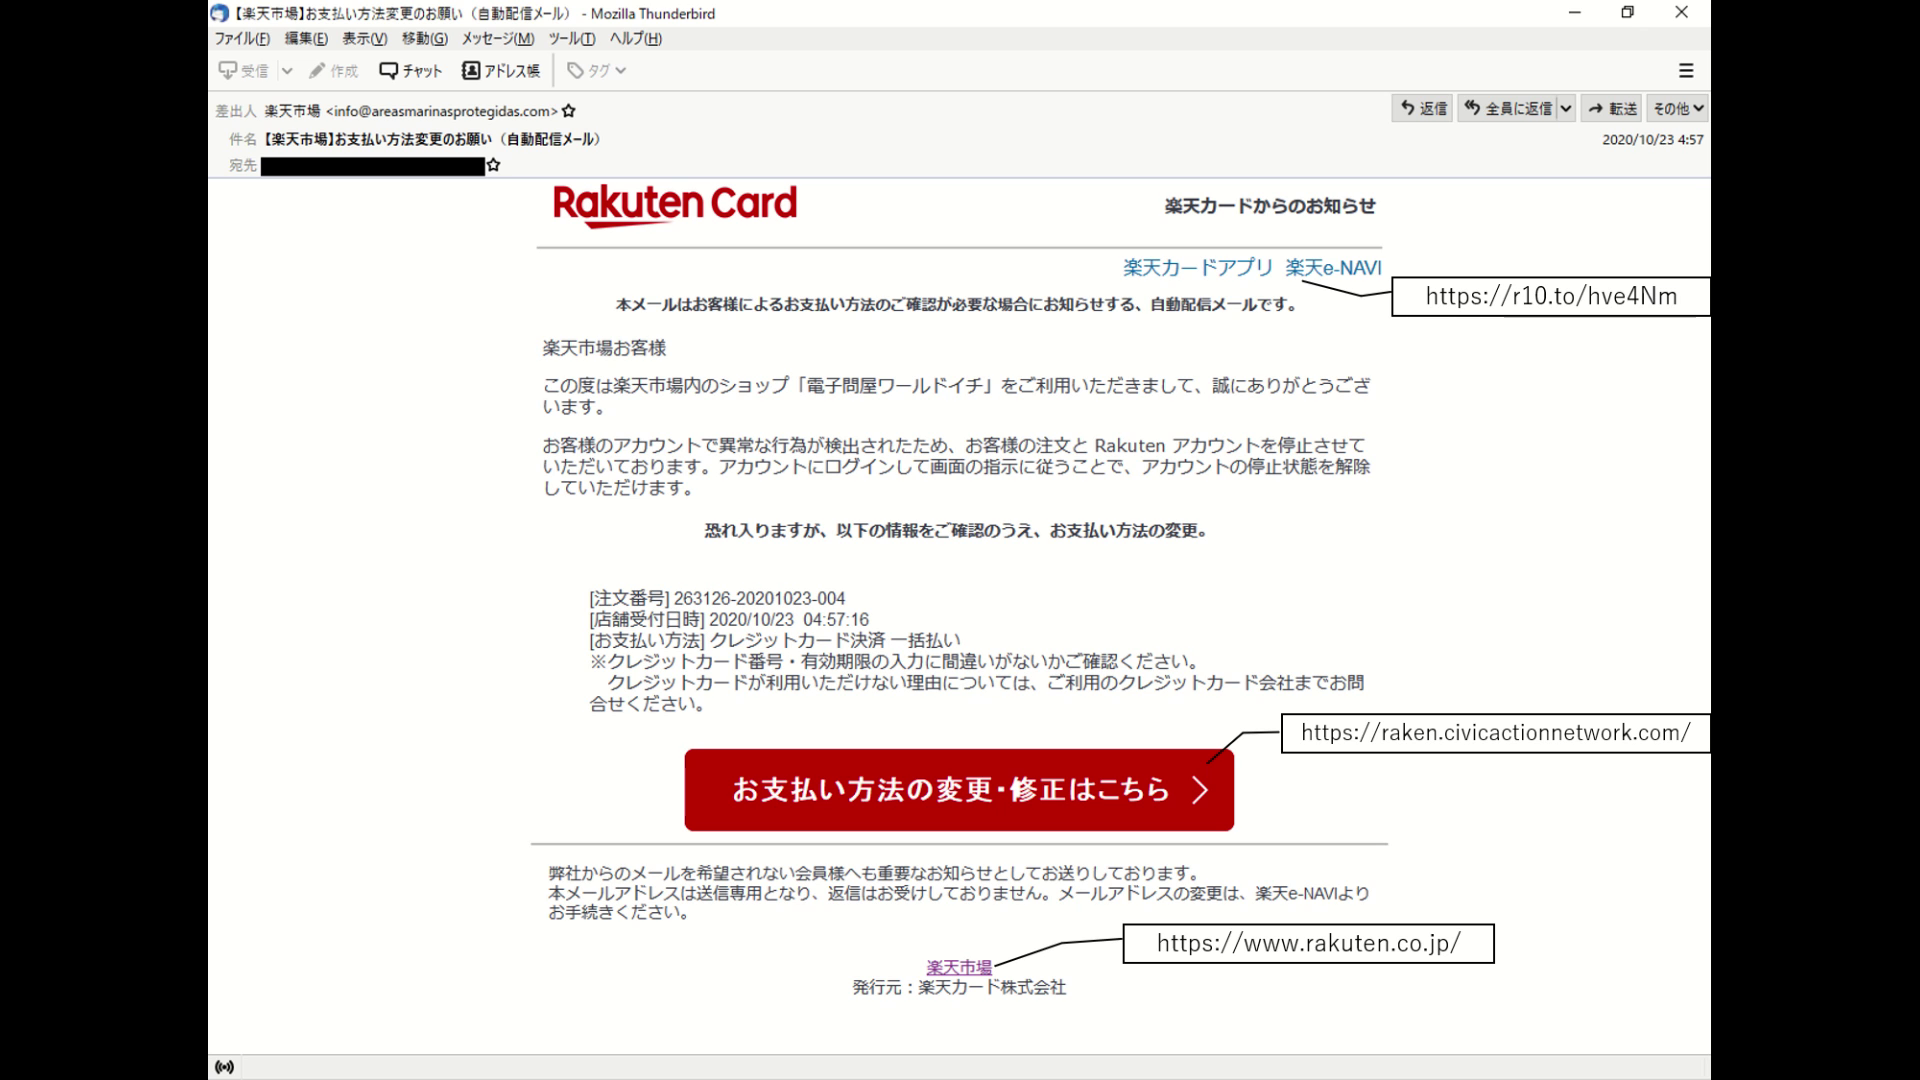
\includegraphics[width=6.5cm]{img/stimuli/06_Rakuten_F_Stim.png}
		\caption{06\_Rakuten\_F\_Stim.png}
		\label{fig:a6}
	\end{minipage}
\end{figure}

\begin{figure}[H]
	\centering
	\begin{minipage}{0.45\linewidth}
		\centering
		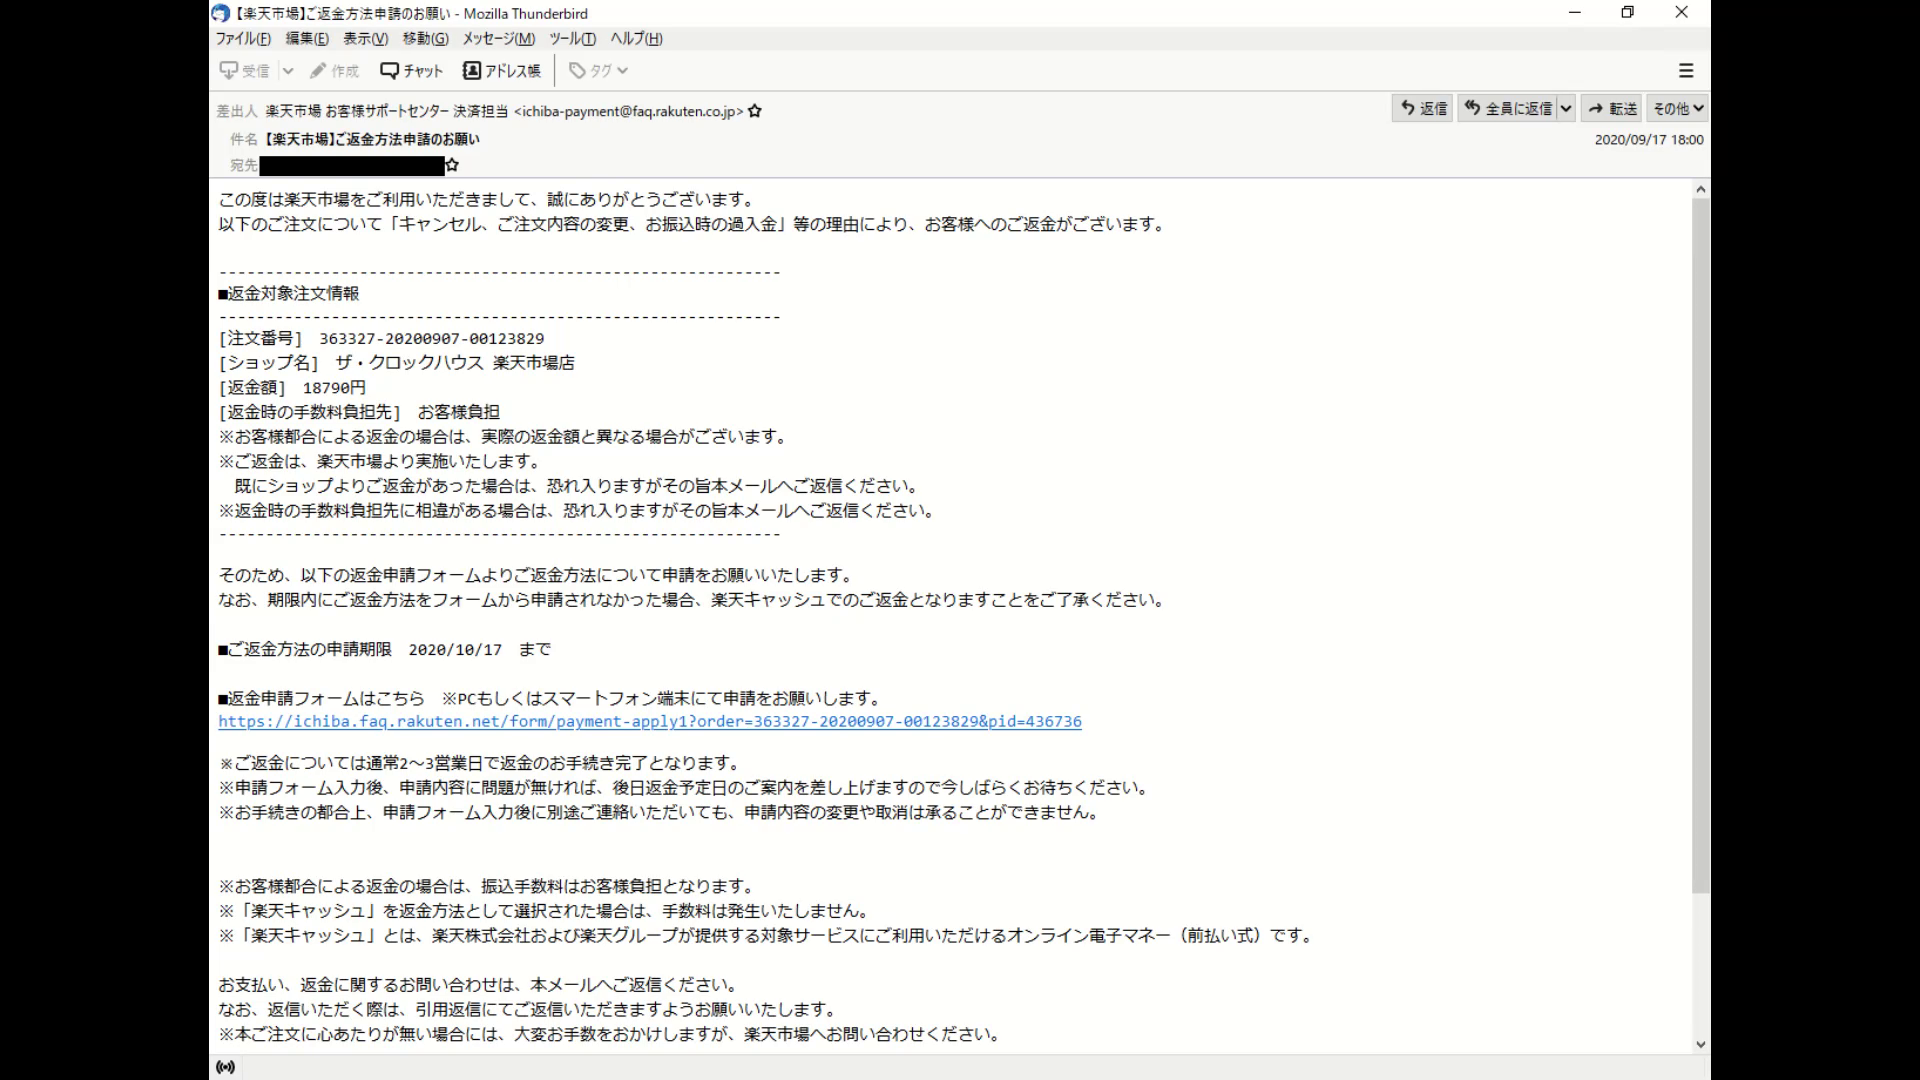
\includegraphics[width=6.5cm]{img/stimuli/07_Rakuten_T_Stim.png}
		\caption{07\_Rakuten\_T\_Stim.png}
		\label{fig:a7}
	\end{minipage}
	\begin{minipage}{0.45\linewidth}
		\centering
		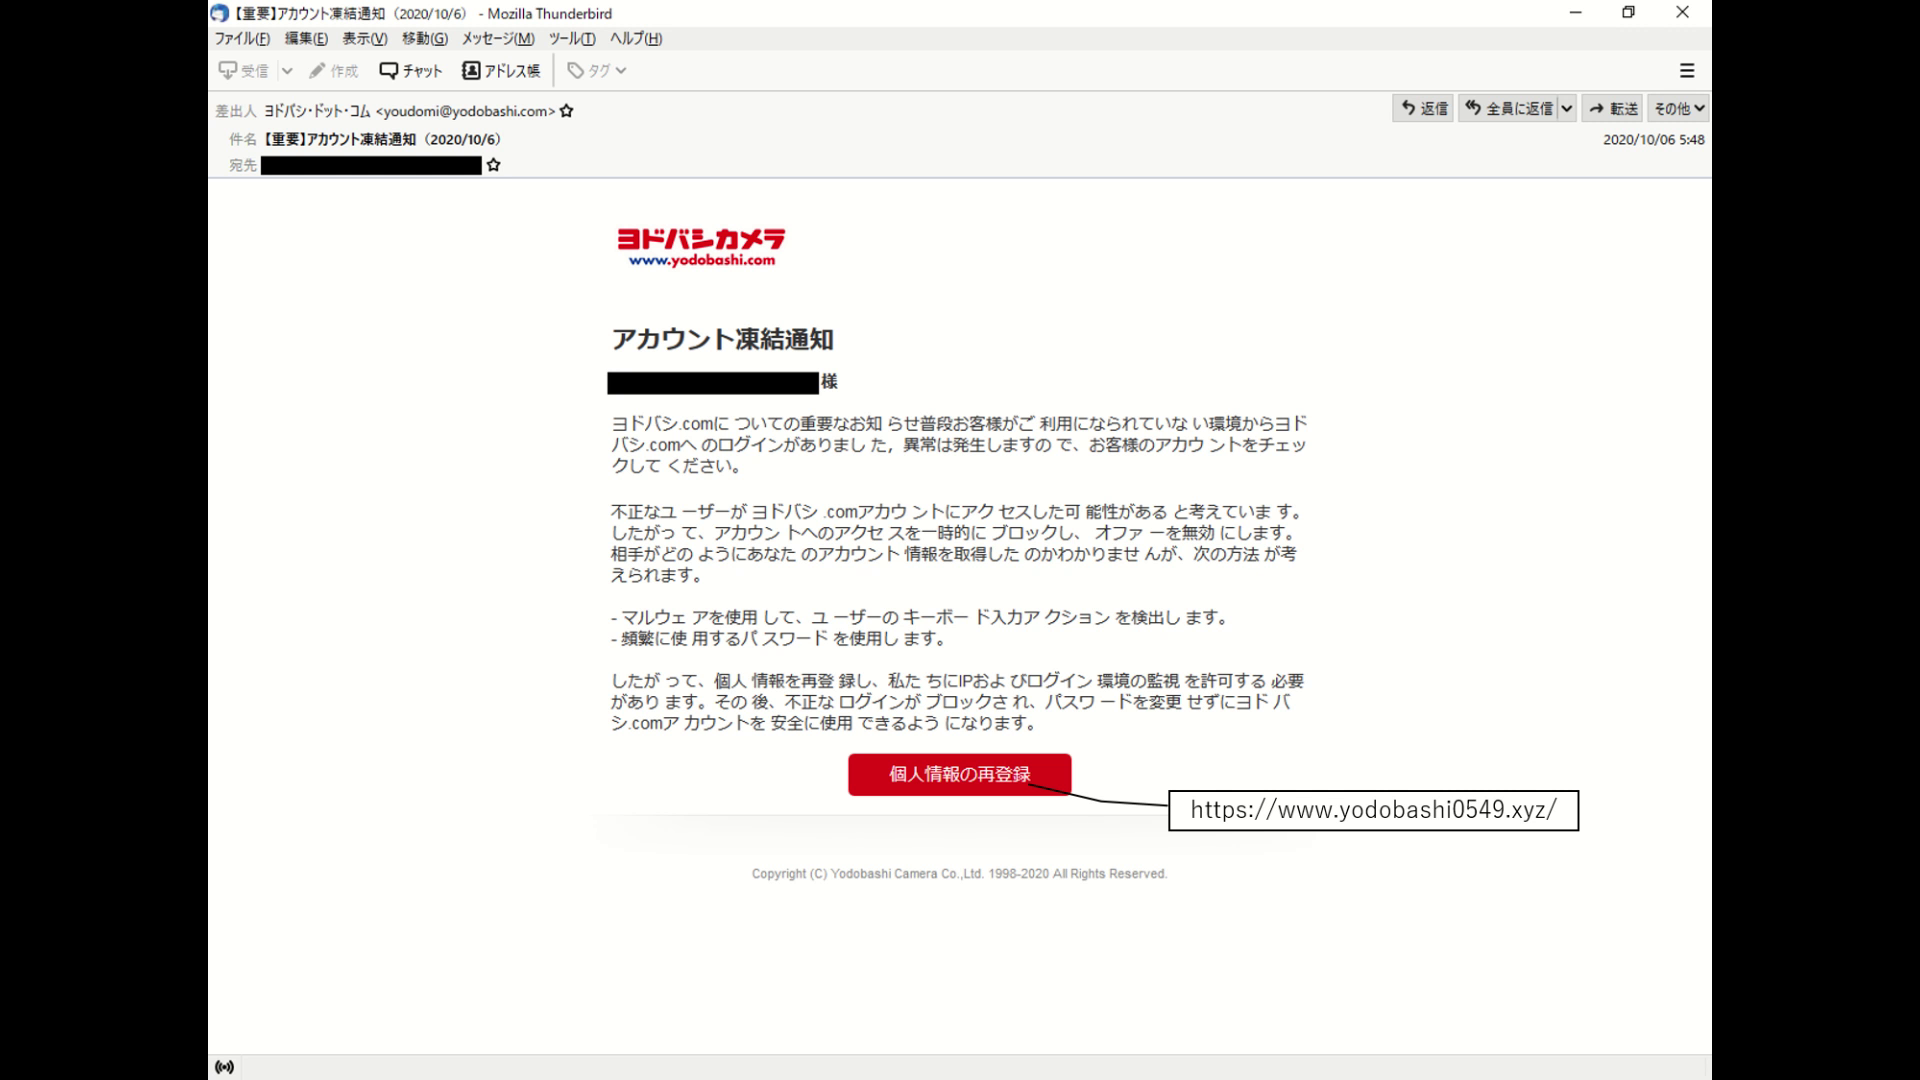
\includegraphics[width=6.5cm]{img/stimuli/08_yodobasi_F_Stim.png}
		\caption{08\_yodobasi\_F\_Stim.png}
		\label{fig:a8}
	\end{minipage}
\end{figure}

\begin{figure}[H]
	\centering
	\begin{minipage}{0.45\linewidth}
		\centering
		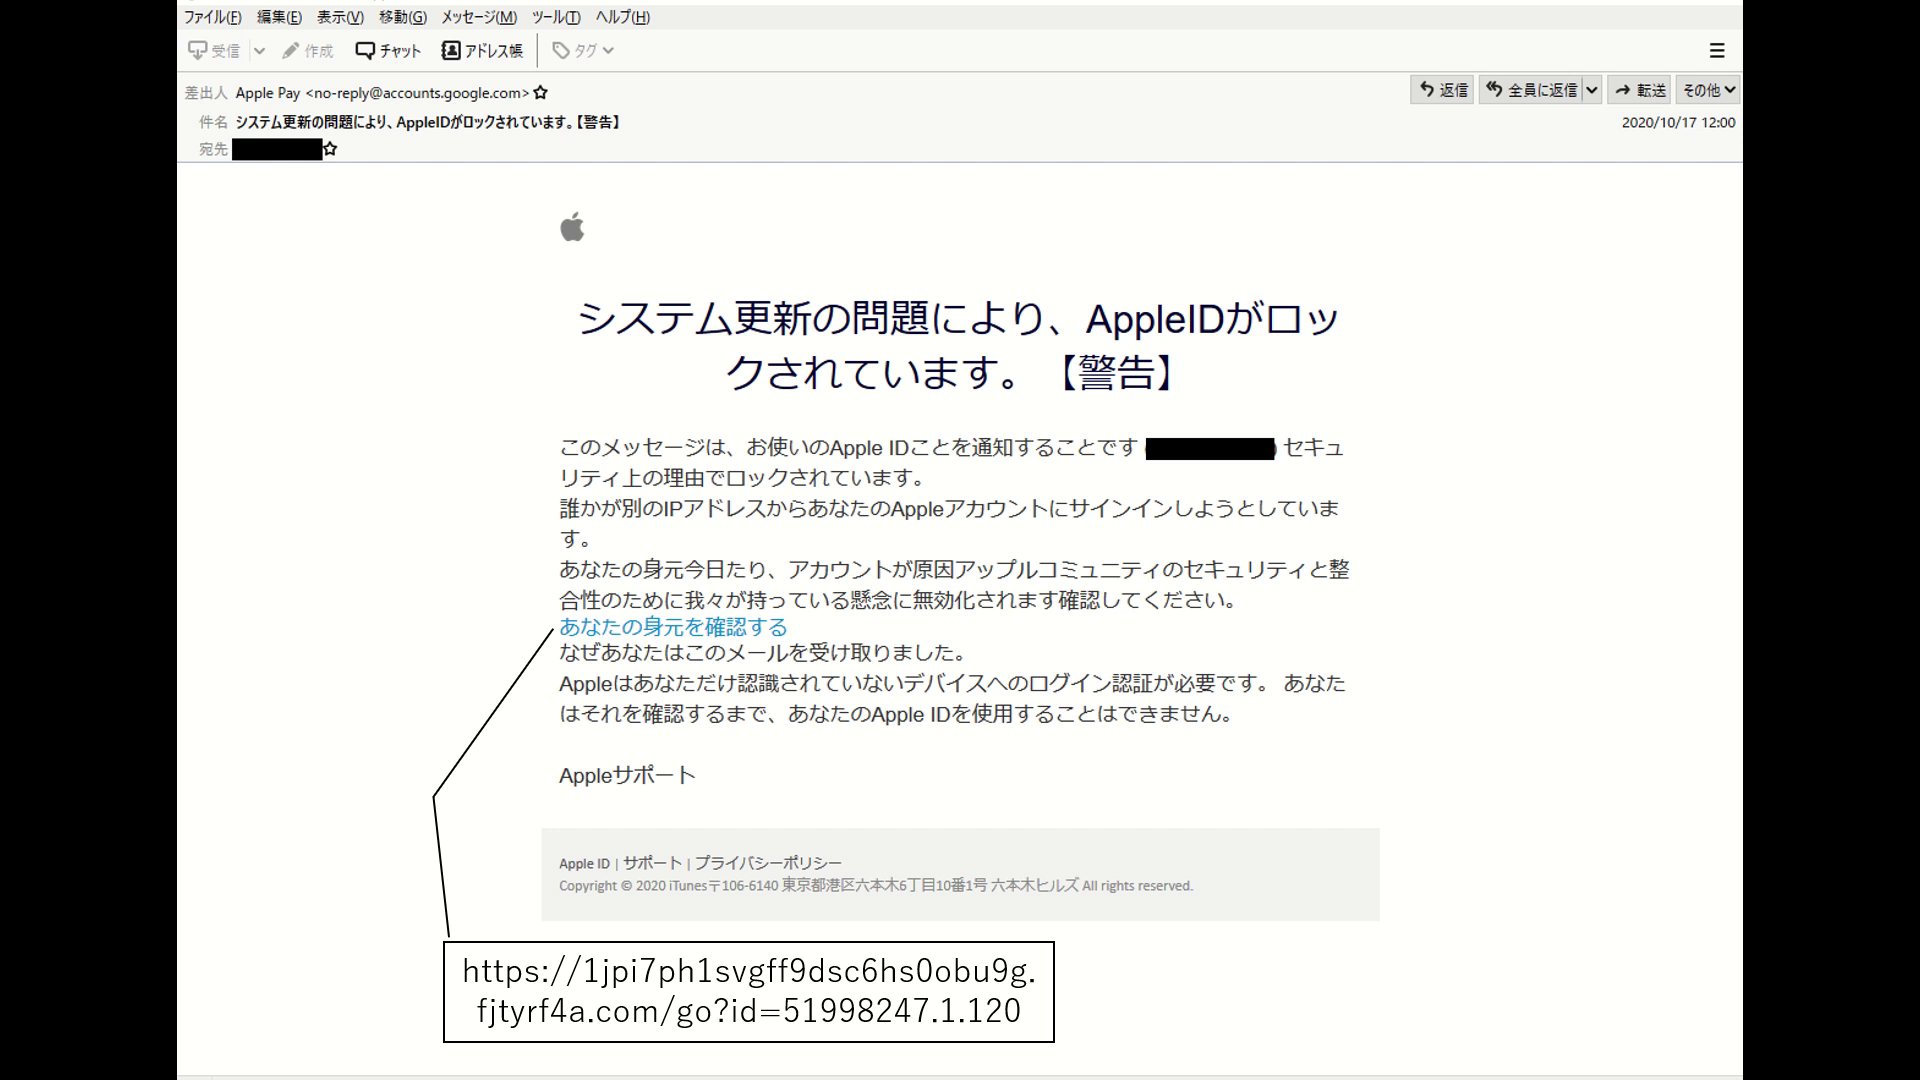
\includegraphics[width=6.5cm]{img/stimuli/09_Apple1_F_Stim.png}
		\caption{09\_Apple1\_F\_Stim.png}
		\label{fig:a9}
	\end{minipage}
	\begin{minipage}{0.45\linewidth}
		\centering
		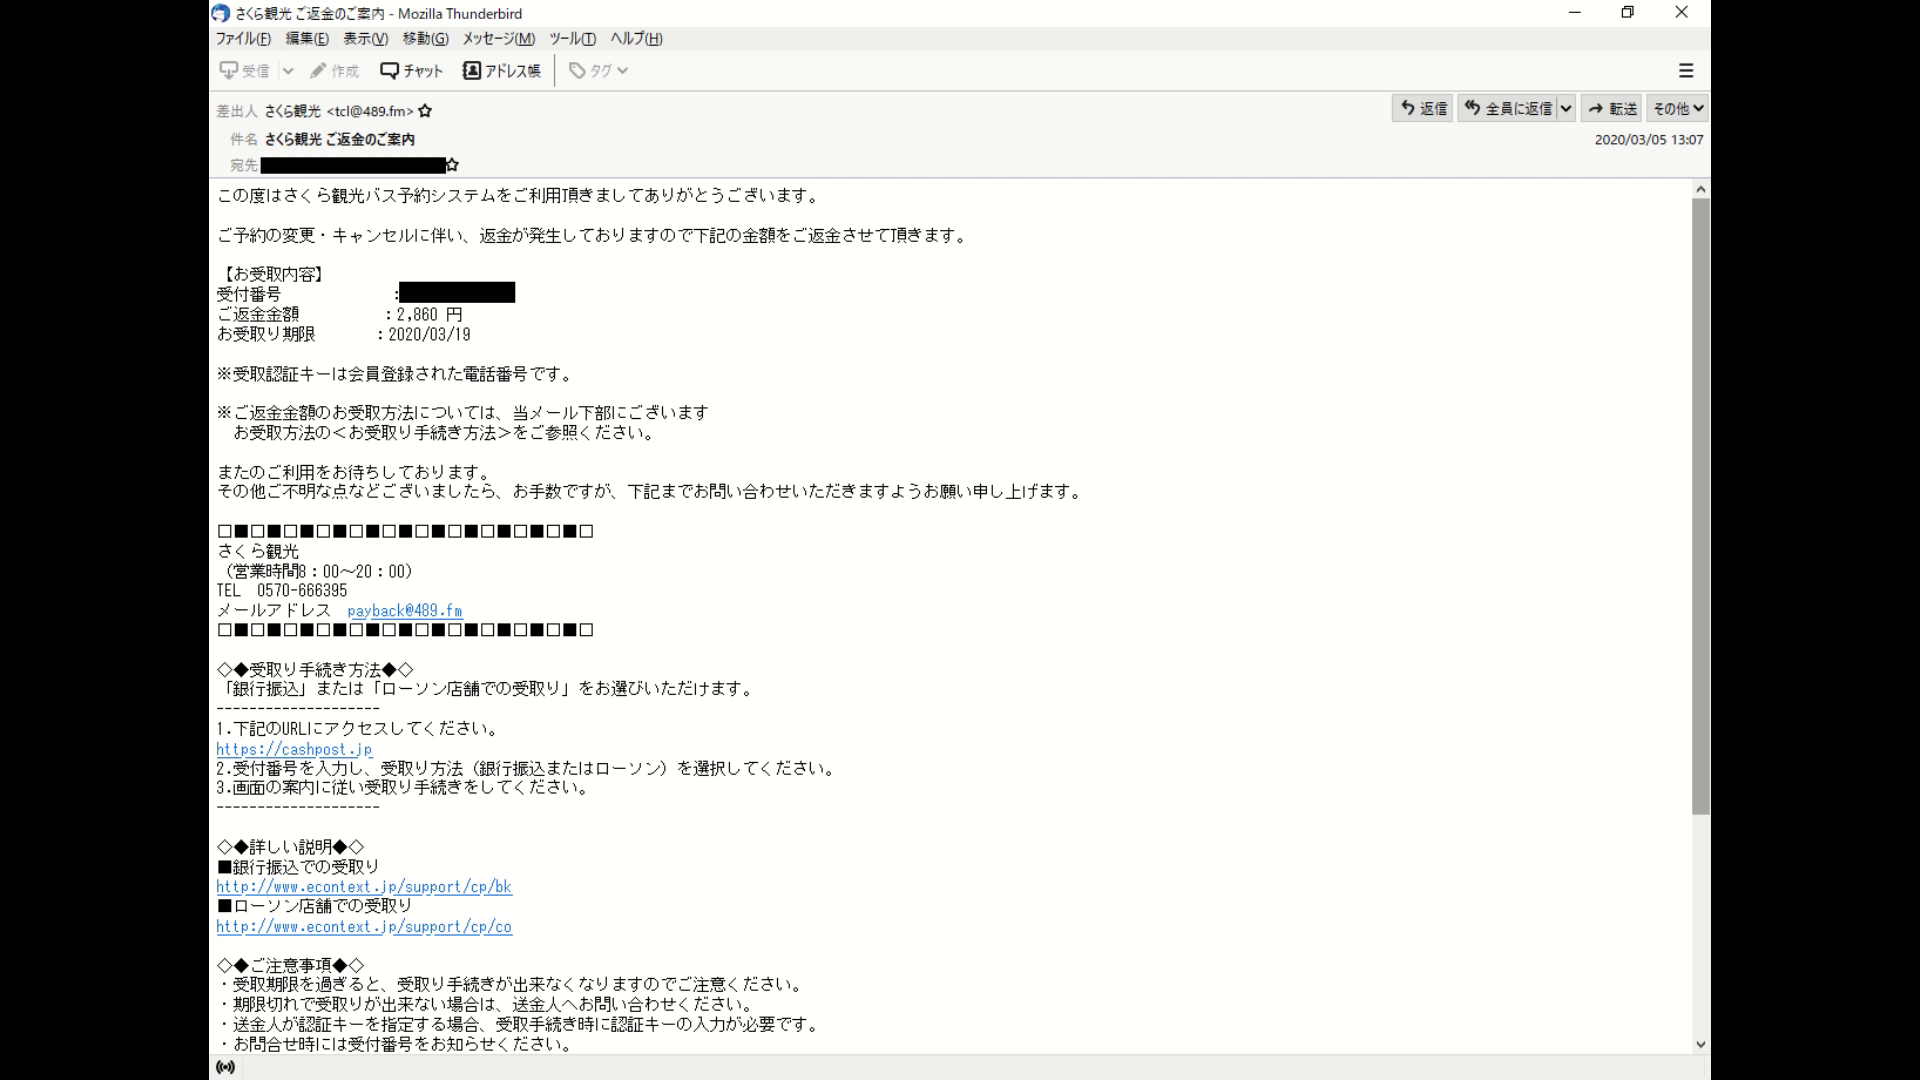
\includegraphics[width=6.5cm]{img/stimuli/10_Kankou_T_Stim.png}
		\caption{10\_Kankou\_T\_Stim.png}
		\label{fig:a10}
	\end{minipage}
\end{figure}

\begin{figure}[H]
	\centering
	\begin{minipage}{0.45\linewidth}
		\centering
		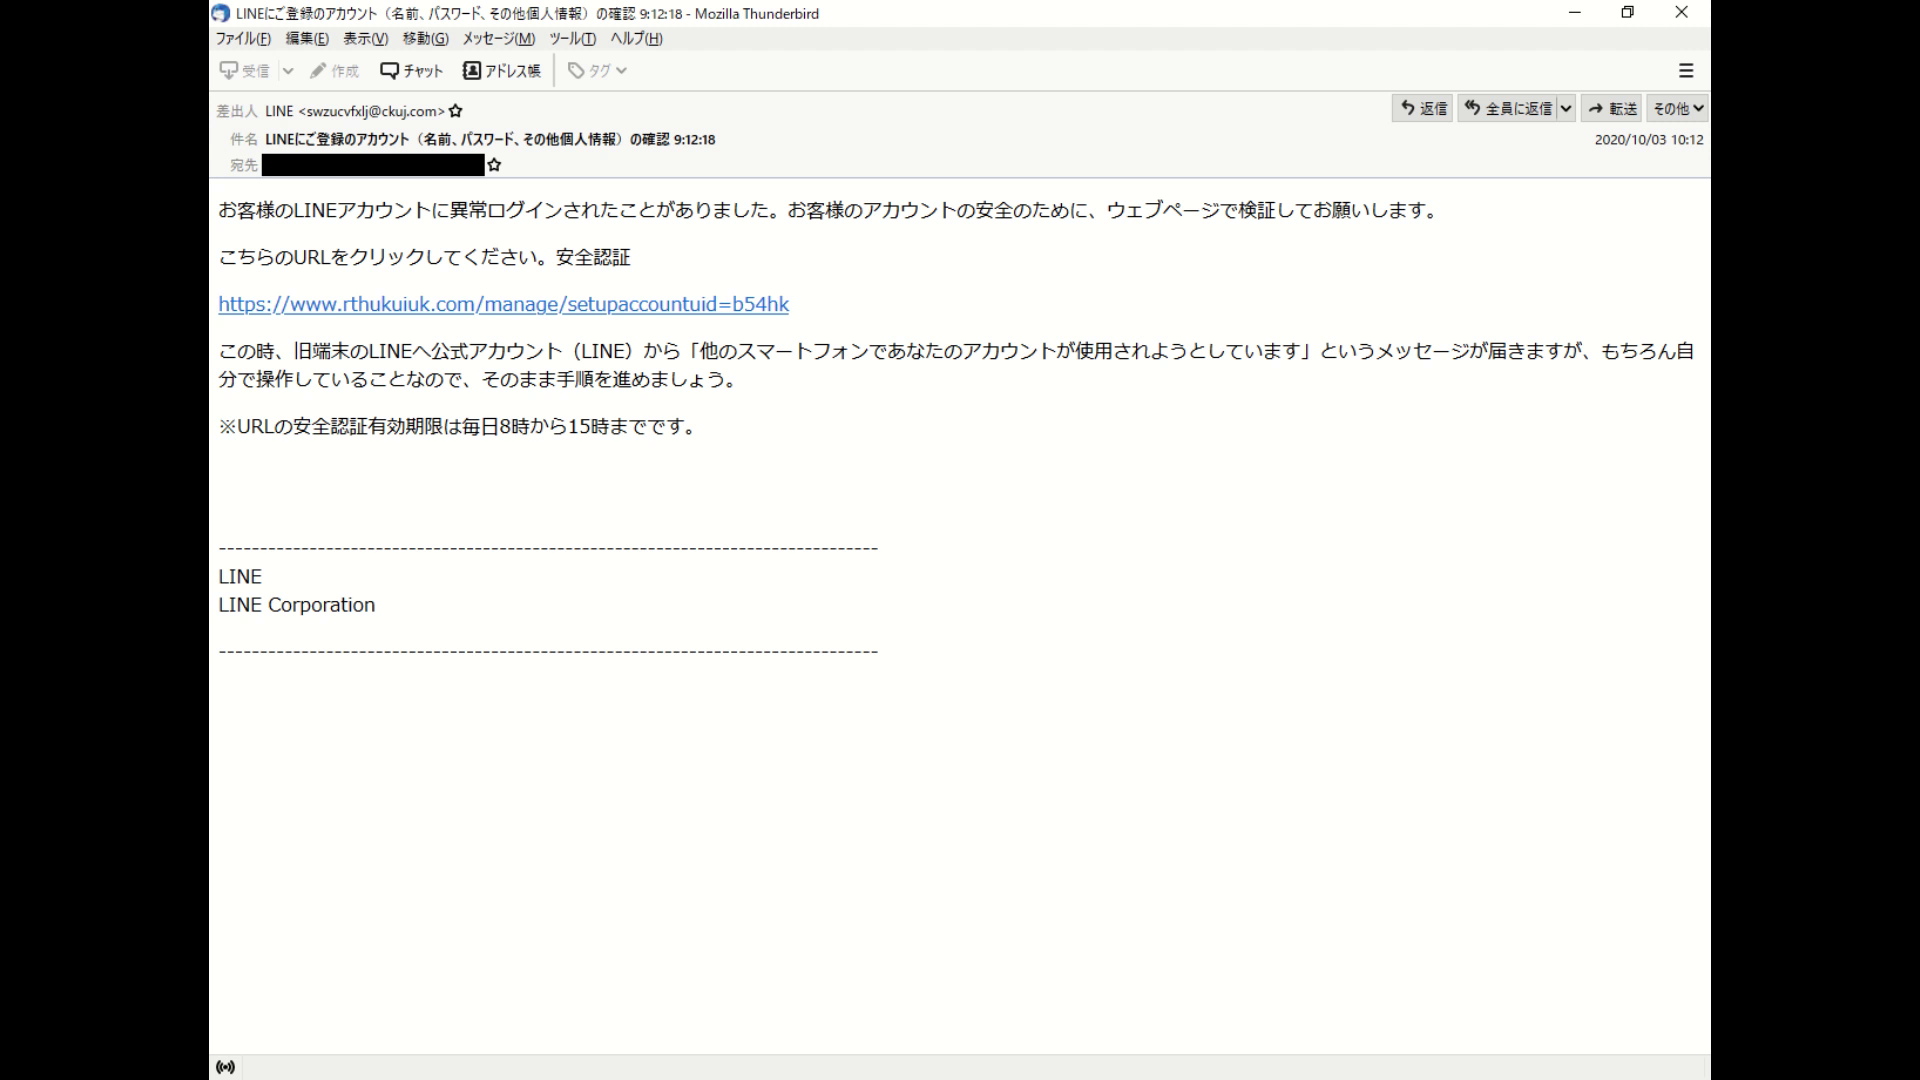
\includegraphics[width=6.5cm]{img/stimuli/11_LINE_F_Stim.png}
		\caption{11\_LINE\_F\_Stim.png}
		\label{fig:a11}
	\end{minipage}
	\begin{minipage}{0.45\linewidth}
		\centering
		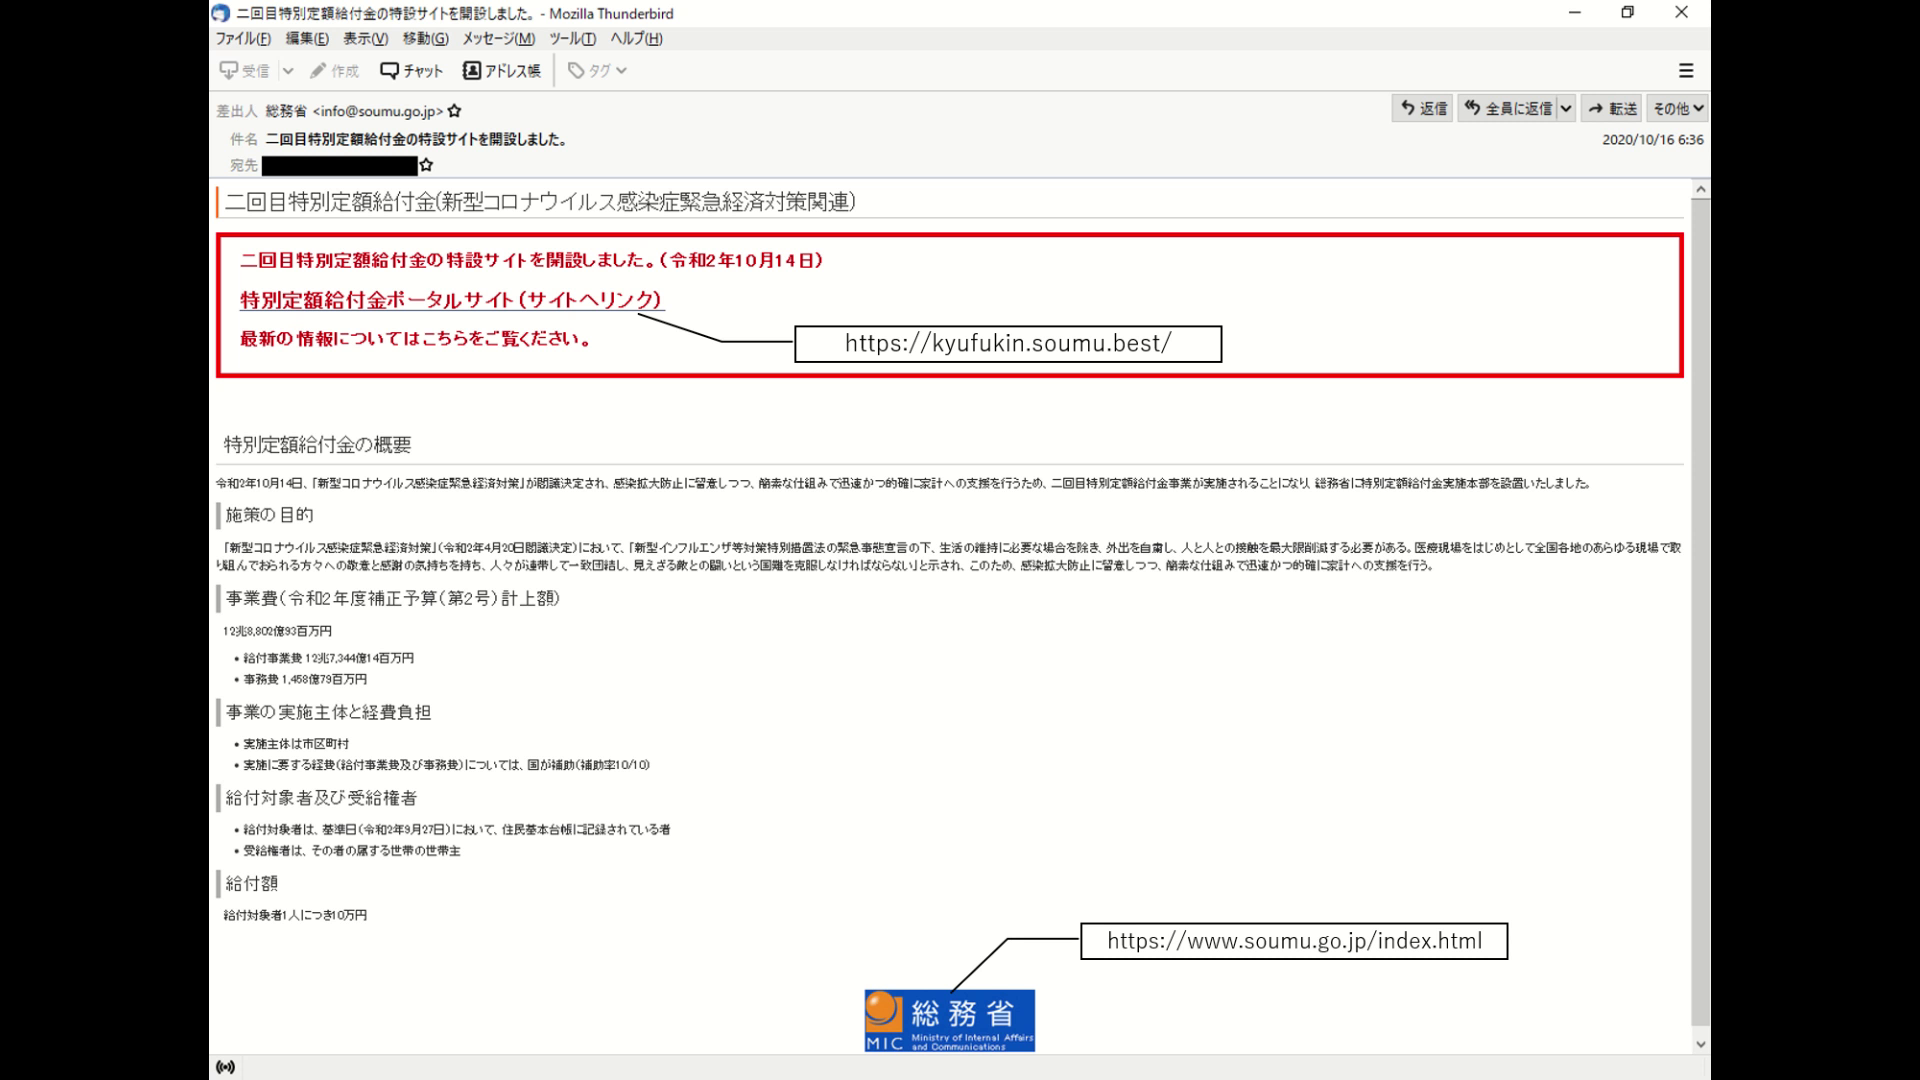
\includegraphics[width=6.5cm]{img/stimuli/12_Kyufu2_F_Stim.png}
		\caption{12\_Kyufu2\_F\_Stim.png}
		\label{fig:a12}
	\end{minipage}
\end{figure}

\begin{figure}[H]
	\centering
	\begin{minipage}{0.45\linewidth}
		\centering
		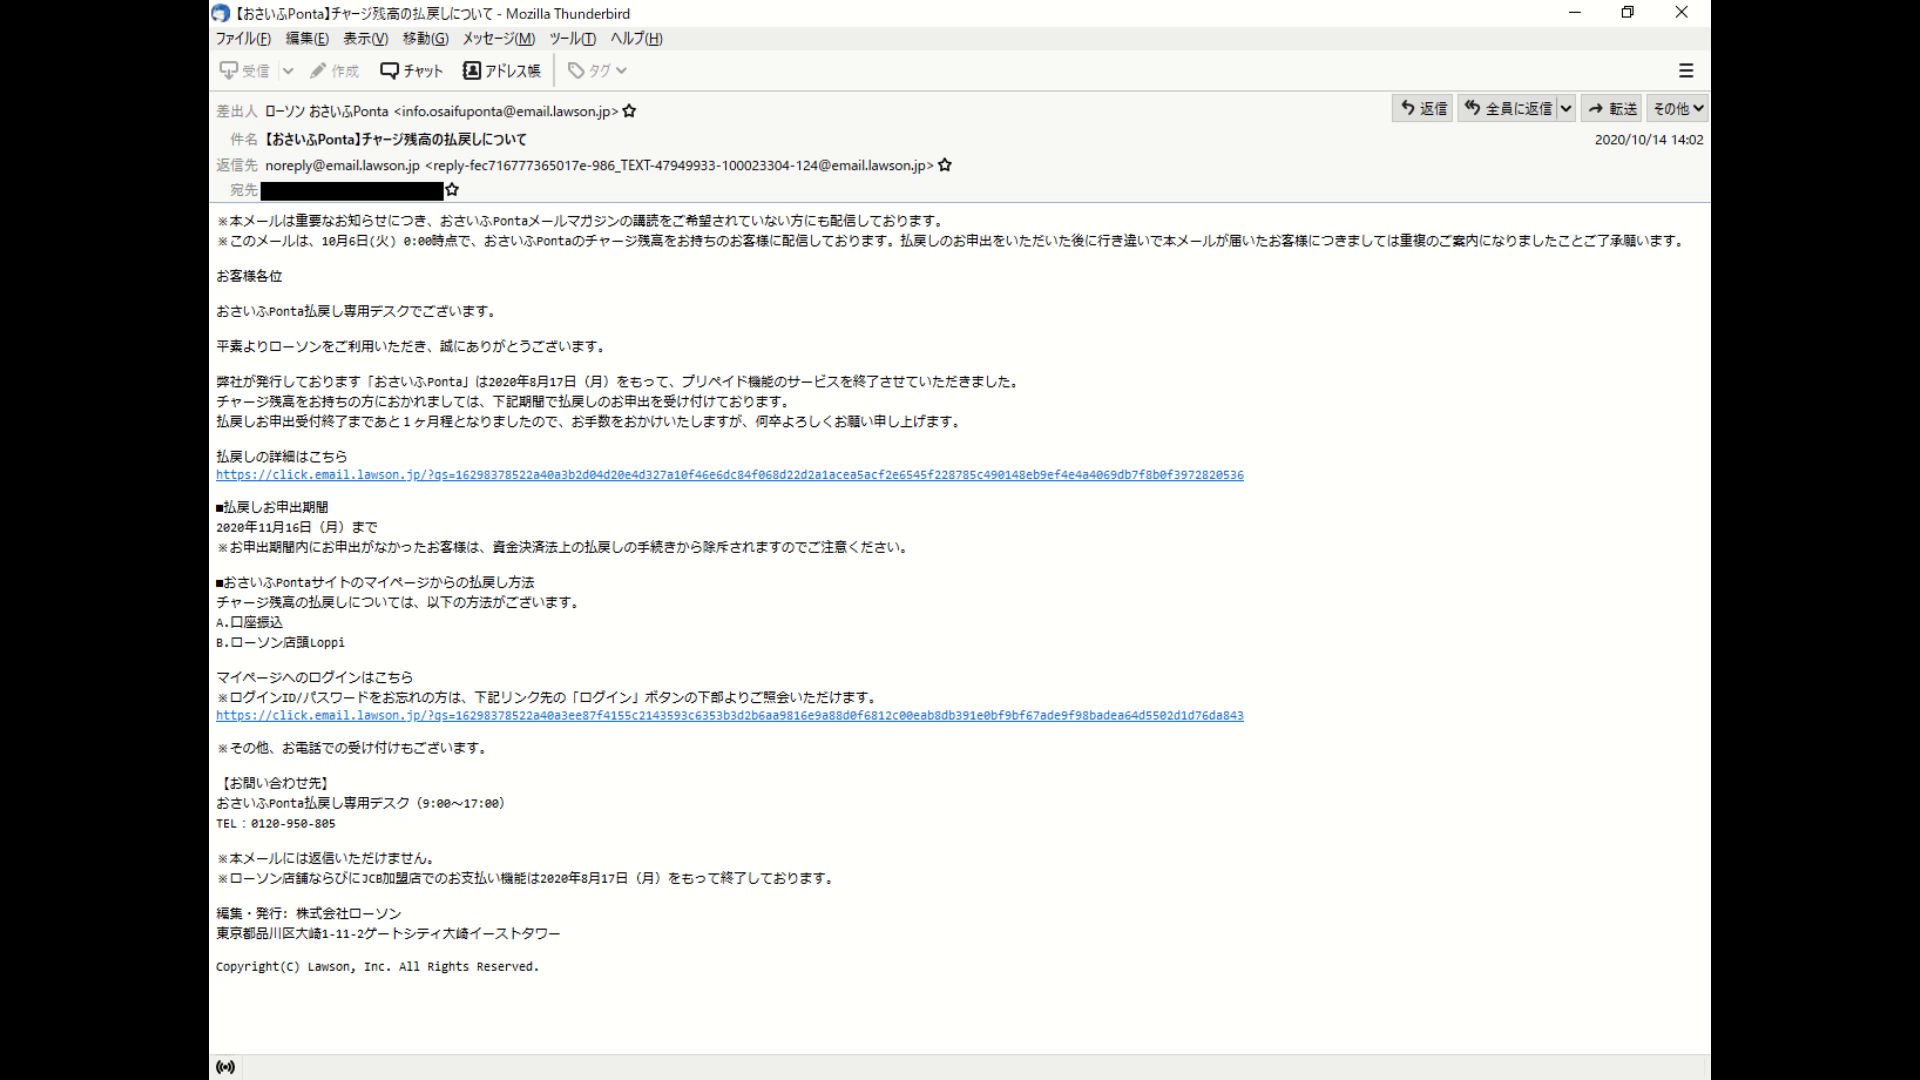
\includegraphics[width=6.5cm]{img/stimuli/13_ponta_T_Stim.png}
		\caption{13\_ponta\_T\_Stim.png}
		\label{fig:a13}
	\end{minipage}
	\begin{minipage}{0.45\linewidth}
		\centering
		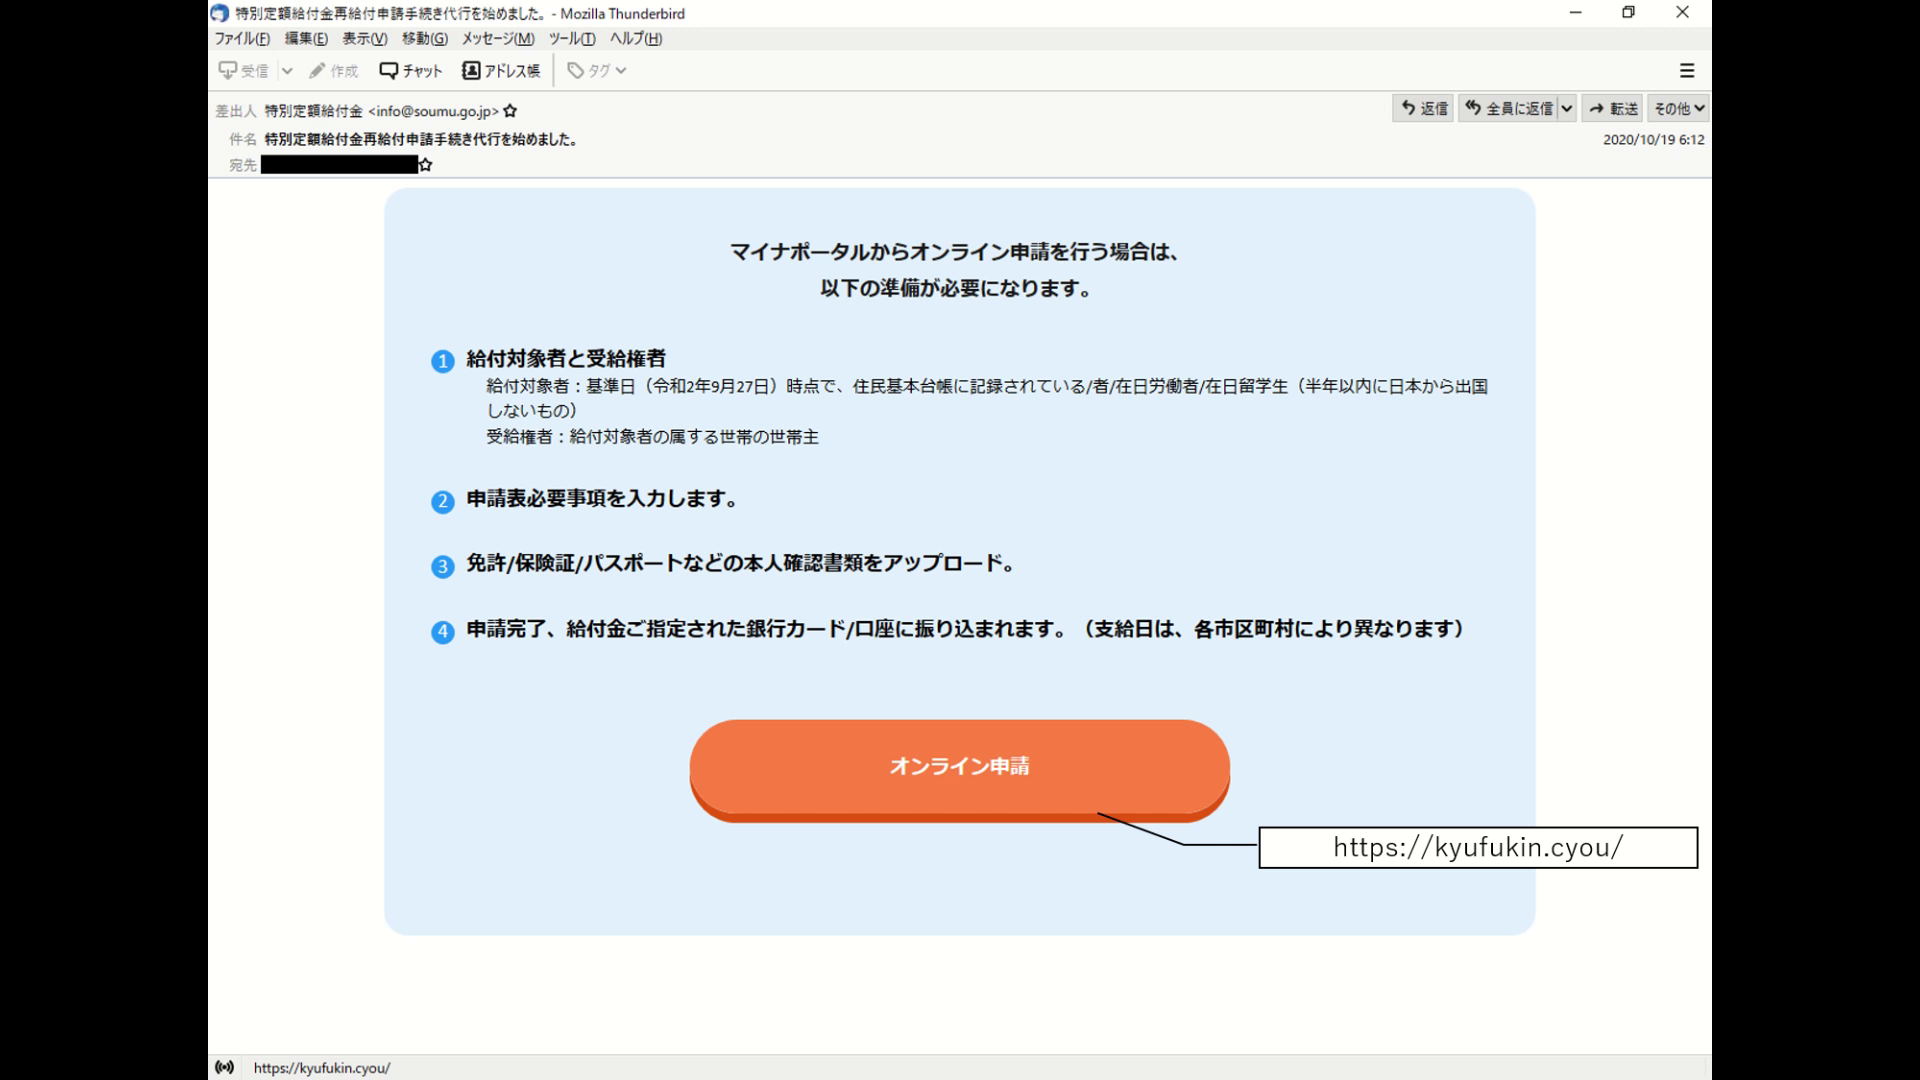
\includegraphics[width=6.5cm]{img/stimuli/14_Kyufu_F_Stim.png}
		\caption{14\_Kyufu\_F\_Stim.png}
		\label{fig:a14}
	\end{minipage}
\end{figure}

\begin{figure}[H]
	\centering
	\begin{minipage}{0.45\linewidth}
		\centering
		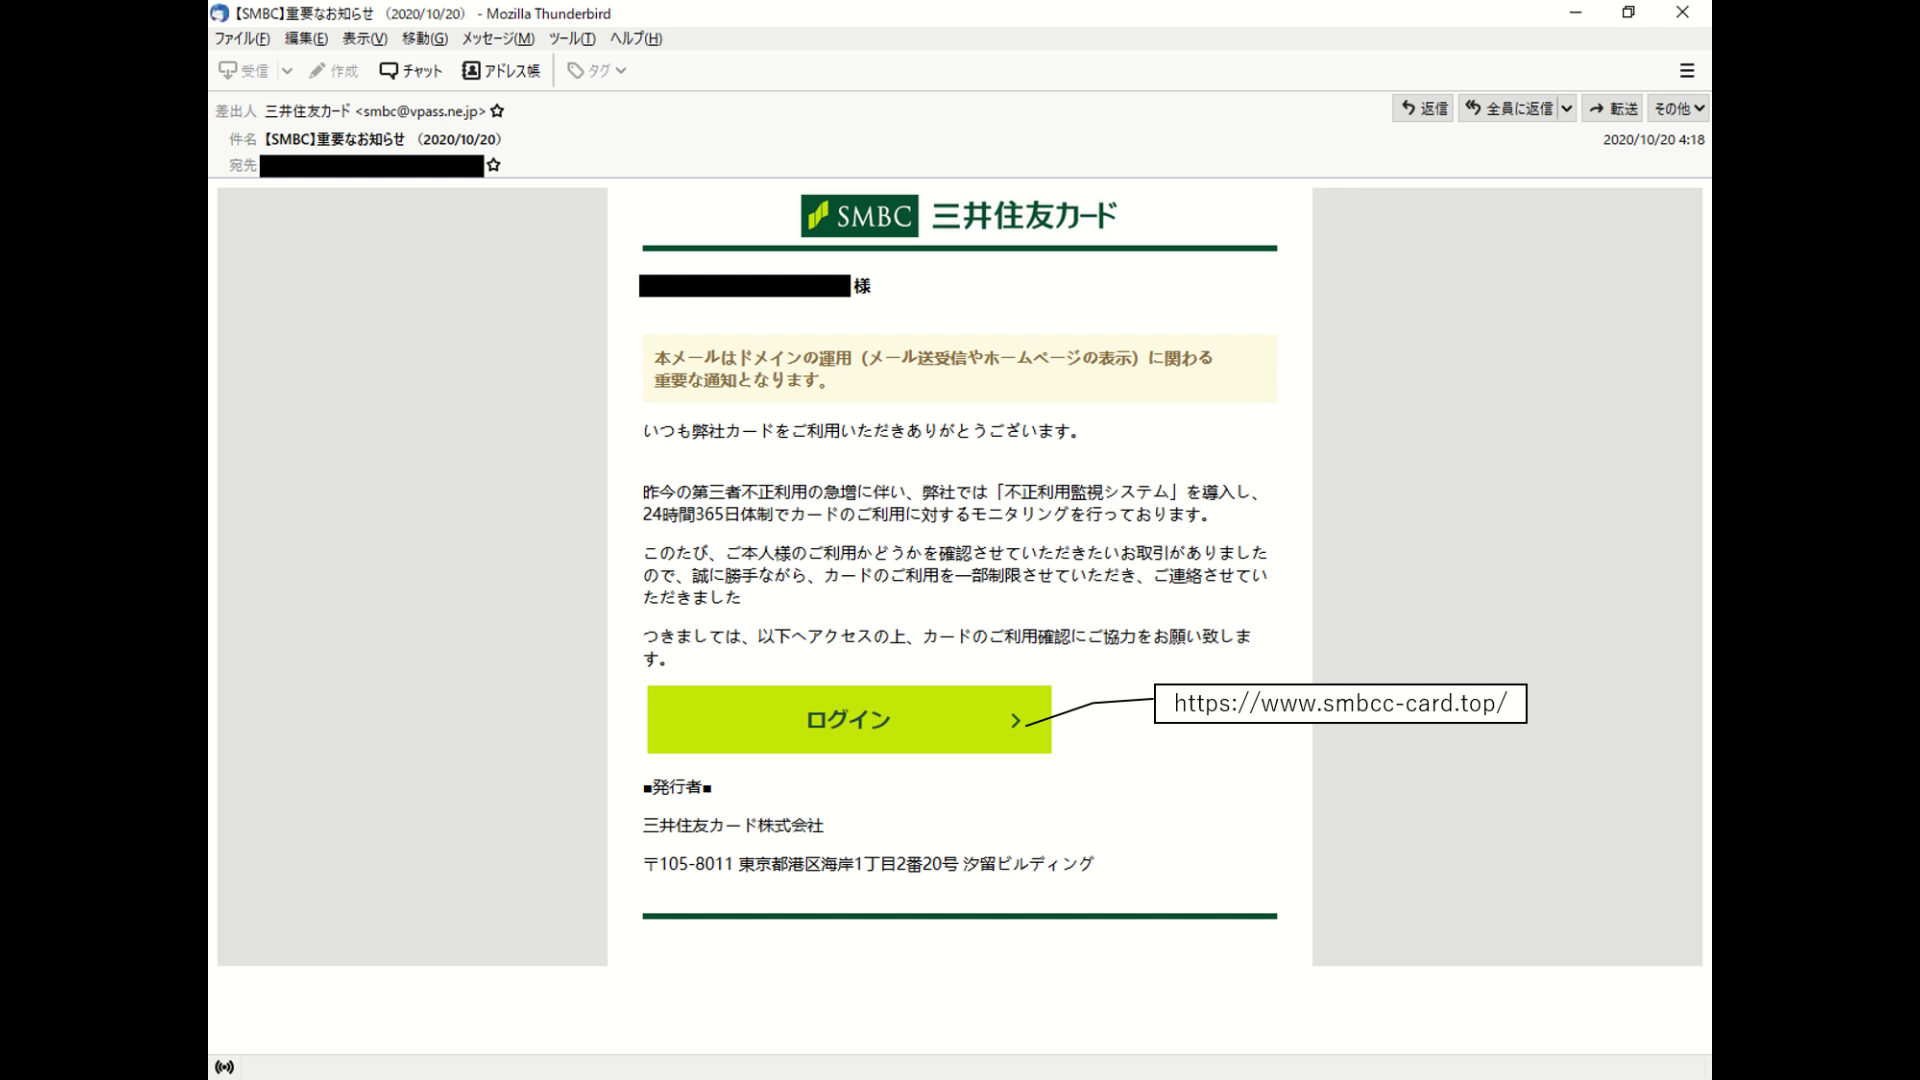
\includegraphics[width=6.5cm]{img/stimuli/15_SMBC_F_Stim.png}
		\caption{15\_SMBC\_F\_Stim.png}
		\label{fig:a15}
	\end{minipage}
	\begin{minipage}{0.45\linewidth}
		\hspace{1em}
	\end{minipage}
\end{figure}

\chapter{ソースコード}
\section{課題1}
\begin{code}
	\captionof{listing}{Confusion\_Matrix.py}
	\label{code:py1}
	\lstinputlisting[language=Python, numbers=left, stepnumber=1, breaklines=true, breakindent=10pt, showstringspaces=false, frame=tbrl, framesep=5pt, basicstyle=\ttfamily\scriptsize, commentstyle=\color{green!50!black}, keywordstyle=\color{blue}, tabsize=2, stringstyle=\color{red}, numberstyle=\tiny, captionpos=t]{code/Confusion_Matrix.py}
\end{code}

\section{課題2}
\begin{code}
	\captionof{listing}{ToI.py}
	\label{code:py2}
	\lstinputlisting[language=Python, numbers=left, stepnumber=1, breaklines=true, breakindent=10pt, showstringspaces=false, frame=tbrl, framesep=5pt, basicstyle=\ttfamily\scriptsize, commentstyle=\color{green!50!black}, keywordstyle=\color{blue}, tabsize=2, stringstyle=\color{red}, numberstyle=\tiny, captionpos=t]{code/ToI.py}
\end{code}

\section{課題3}
\begin{code}
	\captionof{listing}{AoI.py}
	\label{code:py3}
	\lstinputlisting[language=Python, numbers=left, stepnumber=1, breaklines=true, breakindent=10pt, showstringspaces=false, frame=tbrl, framesep=5pt, basicstyle=\ttfamily\scriptsize, commentstyle=\color{green!50!black}, keywordstyle=\color{blue}, tabsize=2, stringstyle=\color{red}, numberstyle=\tiny, captionpos=t]{code/AoI.py}
\end{code}

\begin{code}
	\captionof{listing}{concat.py}
	\label{code:py4}
	\lstinputlisting[language=Python, numbers=left, stepnumber=1, breaklines=true, breakindent=10pt, showstringspaces=false, frame=tbrl, framesep=5pt, basicstyle=\ttfamily\scriptsize, commentstyle=\color{green!50!black}, keywordstyle=\color{blue}, tabsize=2, stringstyle=\color{red}, numberstyle=\tiny, captionpos=t]{code/concat.py}
\end{code}

\section{課題4}
\begin{code}
	\captionof{listing}{Correlation\_analysis.py}
	\label{code:py5}
	\lstinputlisting[language=Python, numbers=left, stepnumber=1, breaklines=true, breakindent=10pt, showstringspaces=false, frame=tbrl, framesep=5pt, basicstyle=\ttfamily\scriptsize, commentstyle=\color{green!50!black}, keywordstyle=\color{blue}, tabsize=2, stringstyle=\color{red}, numberstyle=\tiny, captionpos=t]{code/correlation_analysis.py}
\end{code}

\end{document}